\documentclass[11pt,twoside]{book}

%% include commands for bios, titles etc used in multiple documents
% $Date$
% $Revision$
% $Author$

%%%%%%%%%%%%%%%%%%%%%%%%%%%%%%%%%%%%%%%%%%%%%%%%%%%%%%%%%%%%%%%%%%%%%%%%%%%%%%%%%%%%%%%%%%%%%%%%%%%
%                                                                                                 %
% The mathematical style of these documents follows                                               %
%                                                                                                 %
% A. Thompson and B.N. Taylor. The NIST Guide for the Use of the International System of Units.   %
%    NIST Special Publication 881, 2008.                                                          %
%                                                                                                 %
% http://www.nist.gov/pml/pubs/sp811/index.cfm                                                    %
%                                                                                                 %
%%%%%%%%%%%%%%%%%%%%%%%%%%%%%%%%%%%%%%%%%%%%%%%%%%%%%%%%%%%%%%%%%%%%%%%%%%%%%%%%%%%%%%%%%%%%%%%%%%%

% Packages which force the use of better TeX coding
% Mostly from http://tex.stackexchange.com/q/19264
%%\RequirePackage[l2tabu, orthodox]{nag}
%%\usepackage{fixltx2e}
%\usepackage{isomath} % Disabled for the moment because it changes the syntax for bold and roman Greek math symbols
%%\usepackage[all,warning]{onlyamsmath}
%\usepackage{strict} % Commented out for now because it is uncommon. A copy of style.sty is in Manuals/LaTeX_Style_Files/.

\usepackage{times,mathptmx}
\usepackage[pdftex]{graphicx}
\usepackage{tabularx}
\usepackage{multirow}
\usepackage{pdfsync}
\usepackage{tikz}
\usepackage{pgfplots}
%\pgfplotsset{compat=1.7}
\usepackage{tocloft}
\usepackage{color}
\usepackage{amsmath}
\definecolor{linknavy}{rgb}{0,0,0.50196}
\definecolor{linkred}{rgb}{1,0,0}
\definecolor{linkblue}{rgb}{0,0,1}
\usepackage{float}
\usepackage{caption}
\usepackage{graphpap}
\usepackage{rotating}
\usepackage{geometry}
\usepackage{relsize}
\usepackage{longtable}
\usepackage{lscape}
\usepackage{amssymb}
\usepackage{makeidx} % Create index at end of document
\usepackage[nottoc,notlof,notlot]{tocbibind} % Put the bibliography and index in the ToC
\usepackage{lastpage} % Automatic last page number reference.
\usepackage[T1]{fontenc}
\usepackage{enumerate}
\usepackage{upquote}
\usepackage{moreverb}
\usepackage{morefloats}

% Smokeview Version String
\newcommand{\smvversion}{6.5.0}

\newcommand{\nopart}{\expandafter\def\csname Parent-1\endcsname{}} % To fix table of contents in pdf.
\newcommand{\ct}{\tt\small} % eventually will be deprecated due to http://www.tex.ac.uk/cgi-bin/texfaq2html?label=2letterfontcmd
\newcommand{\textct}[1]{\texttt{\small #1}}

\usepackage{tocstyle} % Fix table of contents sections from overlapping section titles
\usetocstyle{standard}
\usepackage{siunitx}
\sisetup{
    detect-all = true,
    input-decimal-markers = {.},
    input-ignore = {,},
    inter-unit-product = \ensuremath{{}\cdot{}},
    multi-part-units = repeat,
    number-unit-product = \text{~},
    per-mode = fraction,
    separate-uncertainty = true,
}

\usepackage{listings}
\usepackage{textcomp}
\definecolor{lbcolor}{rgb}{0.96,0.96,0.96}
\lstset{
    %backgroundcolor=\color{lbcolor},
    tabsize=4,
    rulecolor=,
    language=Fortran,
        basicstyle=\footnotesize\ttfamily,
        upquote=true,
        aboveskip={\baselineskip},
        belowskip={\baselineskip},
        columns=fixed,
        extendedchars=true,
        breaklines=true,
        breakatwhitespace=true,
        frame=none,
        showtabs=false,
        showspaces=false,
        showstringspaces=false,
        identifierstyle=\ttfamily,
        keywordstyle=\color[rgb]{0,0,0},
        commentstyle=\color[rgb]{0,0,0},
        stringstyle=\color[rgb]{0,0,0},
}

\usepackage{xr-hyper}
\usepackage[pdftex,
        colorlinks=true,
        urlcolor=linkblue,     % \href{...}{...} external (URL)
        citecolor=linkred,     % citation number colors
        linkcolor=linknavy,    % \ref{...} and \pageref{...}
        pdfproducer={pdflatex},
        pagebackref,
        pdfpagemode=UseNone,
        bookmarksopen=true,
        plainpages=false,
        verbose]{hyperref}

% The Following commented code makes the ``Draft'' watermark on each page.
%\usepackage{eso-pic}
%\usepackage{type1cm}
%\makeatletter
%   \AddToShipoutPicture{
%     \setlength{\@tempdimb}{.5\paperwidth}
%     \setlength{\@tempdimc}{.5\paperheight}
%     \setlength{\unitlength}{1pt}
%     \put(\strip@pt\@tempdimb,\strip@pt\@tempdimc){
%     \makebox(0,0){\rotatebox{45}{\textcolor[gray]{0.75}{\fontsize{8cm}\selectfont{RC6}}}}}
% }
%\makeatother

\setlength{\textwidth}{6.5in}
\setlength{\textheight}{9.0in}
\setlength{\topmargin}{0.in}
\setlength{\headheight}{0.in}
\setlength{\headsep}{0.in}
\setlength{\parindent}{0.25in}
\setlength{\oddsidemargin}{0.0in}
\setlength{\evensidemargin}{0.0in}
\setlength{\leftmargini}{\parindent} % Controls the indenting of the "bullets" in a list
\setlength{\cftsecnumwidth}{0.45in}
\setlength{\cftsubsecnumwidth}{0.5in}
\setlength{\cftfignumwidth}{0.45in}
\setlength{\cfttabnumwidth}{0.45in}

\newcommand{\authortitlesigs}
{
\begin{flushright}
Kevin McGrattan \\
Simo Hostikka \\
Randall McDermott \\
Jason Floyd \\
Craig Weinschenk \\
Kristopher Overholt
\end{flushright}
}

\newcommand{\logosigs}{
\begin{minipage}[b]{6.5in}
\parbox[b]{3.5in}{

\includegraphics[width=1.3in]{../Bibliography/VTT_BLACK_L} \\
VTT Technical Research Centre of Finland}
\hfill
\parbox[b]{3in}{\flushright{
\includegraphics[width=2.in]{../Bibliography/nistident_flright_vec}}}
\end{minipage}
}

\newcommand{\authorsigs}
{
\begin{flushright}
Kevin McGrattan \\
Randall McDermott \\
{\em Fire Research Division \\
Engineering Laboratory \\
Gaithersburg, Maryland, USA} \\[.1in]
Simo Hostikka \\
{\em Aalto University \\
Espoo, Finland} \\[.1in]
Jason Floyd \\
Craig Weinschenk \\
{\em Jensen Hughes \\
Baltimore, Maryland, USA}\\[.1in]
Kristopher Overholt \\
{\em Continuum Analytics \\
Austin, Texas, USA}
\end{flushright}
}

\newcommand{\titlesigs}
{
\small
\begin{flushright}
U.S. Department of Commerce \\
{\em Wilbur L. Ross, Jr., Secretary} \\
\hspace{1in} \\
National Institute of Standards and Technology \\
{\em Kent Rochford, Acting Under Secretary of Commerce for Standards and Technology and Acting NIST Director}
\end{flushright}
}


\newcommand{\disclaimer}[1]{
\begin{minipage}[t][8in][s]{6.5in}
\fontsize{10}{12}\selectfont
\flushright{Certain commercial entities, equipment, or materials may be identified in this \\
document in order to describe an experimental procedure or concept adequately. \\
Such identification is not intended to imply recommendation or endorsement by the \\
National Institute of Standards and Technology, nor is it intended to imply that the \\
entities, materials, or equipment are necessarily the best available for the purpose.\\
}

\vspace{3in}

\large
\flushright{\bf National Institute of Standards and Technology Special Publication #1 \\
Natl.~Inst.~Stand.~Technol.~Spec.~Publ.~#1, \pageref{LastPage} pages (October 2013) \\
CODEN: NSPUE2 }

\vfill

\hspace{1in}

\end{minipage}
}



\newcommand{\gforneybio}
{
\item[Glenn Forney] is a computer scientist at the Engineering Laboratory of NIST.  He received a
bachelor of science degree in mathematics from Salisbury State College and a master of
science and a doctorate in mathematics from Clemson University.  He joined NIST
in 1986 (then the National Bureau of Standards) and has since worked on developing tools that
provide a better understanding of fire phenomena, most notably Smokeview, a software tool for visualizing
Fire Dynamics Simulator data.
}

\newcommand{\smvoverview}
{
This guide is part of a three volume set of companion documents describing how to use Smokeview
in Volume I, the Smokeview User's Guide~\cite{Smokeview_Users_Guide}, describing technical details of how the visualizations are performed in Volume II, the Smokeview Technical Reference Guide~\cite{Smokeview_Tech_Guide}, and presents example cases
verifying the various visualization capabilities of Smokeview in Volume III, the Smokeview Verification Guide~\cite{Smokeview_Verification_Guide}.  Details on the use and technical background of the Fire Dynamics Simulator is contained in the FDS User's~\cite{FDS_Users_Guide} and Technical reference guide~\cite{FDS_Math_Guide}
respectively.
}

% commands to use for "official" cover and title pages
% see smokeview verification guide to see how they are used

\newcommand{\headerA}[1]{
\begin{flushright}
\fontsize{20}{24}\selectfont
\bf{NIST Special Publication #1}
\end{flushright}
}


\newcommand{\headerB}[1]{
\begin{flushright}
\fontsize{28}{33.6}\selectfont
\bf{#1}
\end{flushright}
}

\newcommand{\headerC}[1]{
\vspace{.15in}
\begin{flushright}
\fontsize{12}{14}\selectfont
#1
\end{flushright}
}

\newcommand{\headerD}[1]{
\begin{flushright}
\fontsize{12}{14}\selectfont
http://dx.doi.org/10.6028/NIST.SP.#1
\end{flushright}
}



\newcommand{\dod}[2]{\frac{\partial #1}{\partial #2}}
\newcommand{\DoD}[2]{\frac{\mathrm{D} #1}{\mathrm{D} #2}}
\newcommand{\dsods}[2]{\frac{\partial^2 #1}{\partial #2^2}}
\renewcommand{\d}{\,\mathrm{d}}
\newcommand{\dx}{\delta x}
\newcommand{\dy}{\delta y}
\newcommand{\dz}{\delta z}
\newcommand{\degF}{$^\circ$F}
\newcommand{\degC}{$^\circ$C}
\newcommand{\x}{x}
\newcommand{\y}{y}
\newcommand{\z}{z}
\newcommand{\dt}{\delta t}
\newcommand{\dn}{\delta n}
\newcommand{\cH}{H}
\newcommand{\hu}{u}
\newcommand{\hv}{v}
\newcommand{\hw}{w}
\newcommand{\la}{\lambda}
\newcommand{\bO}{{\Omega}}
\newcommand{\bo}{{\mathbf{\omega}}}
\newcommand{\btau}{\mathbf{\tau}}
\newcommand{\bdelta}{{\mathbf{\delta}}}
\newcommand{\sumyw}{\sum (Y_\alpha/W_\alpha)}
\newcommand{\oW}{\overline{W}}
\newcommand{\om}{\ensuremath{\omega}}
\newcommand{\omx}{\omega_x}
\newcommand{\omy}{\omega_y}
\newcommand{\omz}{\omega_z}
\newcommand{\erf}{\hbox{erf}}
\newcommand{\erfc}{\hbox{erfc}}
\newcommand{\bF}{{\mathbf{F}}}
\newcommand{\bG}{{\mathbf{G}}}
\newcommand{\bof}{{\mathbf{f}}}
\newcommand{\bq}{{\mathbf{q}}}
\newcommand{\br}{{\mathbf{r}}}
\newcommand{\bu}{{\mathbf{u}}}
\newcommand{\bx}{{\mathbf{x}}}
\newcommand{\bk}{{\mathbf{k}}}
\newcommand{\bv}{{\mathbf{v}}}
\newcommand{\bg}{{\mathbf{g}}}
\newcommand{\bn}{{\mathbf{n}}}
\newcommand{\bS}{{\mathbf{S}}}
\newcommand{\bW}{\overline{W}}
\newcommand{\dS}{d{\mathbf{S}}}
\newcommand{\bs}{{\mathbf{s}}}
\newcommand{\bI}{{\mathbf{I}}}
\newcommand{\hp}{H}
\newcommand{\trho}{\tilde{\rho}}
\newcommand{\dph}{{\delta\phi}}
\newcommand{\dth}{{\delta\theta}}
\newcommand{\tp}{\tilde{p}}
\newcommand{\bp}{\overline{p}}
\newcommand{\dQ}{\dot{Q}}
\newcommand{\dq}{\dot{q}}
\newcommand{\dbq}{\dot{\mathbf{q}}}
\newcommand{\dm}{\dot{m}}
\newcommand{\ha}{\frac{1}{2}}
\newcommand{\ft}{\frac{4}{3}}
\newcommand{\ot}{\frac{1}{3}}
\newcommand{\fofi}{\frac{4}{5}}
\newcommand{\of}{\frac{1}{4}}
\newcommand{\twth}{\frac{2}{3}}
\newcommand{\R}{R}
\newcommand{\be}{\begin{equation}}
\newcommand{\ee}{\end{equation}}
\newcommand{\RE}{\hbox{Re}}
\newcommand{\LE}{\hbox{Le}}
\newcommand{\PR}{\hbox{Pr}}
\newcommand{\PE}{\hbox{Pe}}
\newcommand{\NU}{\hbox{Nu}}
\newcommand{\SC}{\hbox{Sc}}
\newcommand{\SH}{\hbox{Sh}}
\newcommand{\WE}{\hbox{We}}
\newcommand{\COTWO}{\text{\tiny \hbox{CO}$_2$}}
\newcommand{\HTWOO}{\text{\tiny \hbox{H}$_2$\hbox{O}}}
\newcommand{\OTWO}{\text{\tiny \hbox{O}$_2$}}
\newcommand{\NTWO}{\text{\tiny \hbox{N}$_2$}}
\newcommand{\CO}{\text{\tiny \hbox{CO}}}
\newcommand{\F}{\text{\tiny \hbox{F}}}
\newcommand{\C}{\text{\tiny \hbox{C}}}
\newcommand{\Hy}{\text{\tiny \hbox{H}}}
\newcommand{\So}{\text{\tiny \hbox{S}}}
\newcommand{\M}{\text{\tiny \hbox{M}}}
\newcommand{\xx}{\text{\tiny \hbox{x}}}
\newcommand{\yy}{\text{\tiny \hbox{y}}}
\newcommand{\zz}{\text{\tiny \hbox{z}}}
\newcommand{\smvlines}{135~000}

\newcommand{\calH}{\mathcal{H}}
\newcommand{\calR}{\mathcal{R}}

\newcommand{\dif}{\mathrm{d}}
\newcommand{\Div}{\nabla\cdot}
\newcommand{\D}{\mbox{D}}
\newcommand{\mhalf}{\mbox{$\frac{1}{2}$}}
\newcommand{\thalf}{\mbox{\tiny $\frac{1}{2}$}}
\newcommand{\tripleprime}{{\prime\prime\prime}}
\newcommand{\ppp}{{\prime\prime\prime}}
\newcommand{\pp}{{\prime\prime}}

\newcommand{\superscript}[1]{\ensuremath{^{\textrm{\tiny #1}}}}
\newcommand{\subscript}[1]{\ensuremath{_{\textrm{\tiny #1}}}}

\newcommand{\rb}[1]{\raisebox{1.5ex}[0pt]{#1}}

\newcommand{\Ra}{$\Rightarrow$}
\newcommand{\hhref}[1]{\href{#1}{{\tt #1}}}
\newcommand{\fdsinput}[1]{{\scriptsize\verbatiminput{../../Verification/Visualization/#1}}}

\definecolor{AQUAMARINE}{rgb}{0.49804,1.00000,0.83137}
\definecolor{ANTIQUE WHITE}{rgb}{0.98039,0.92157,0.84314}
\definecolor{BEIGE}{rgb}{0.96078,0.96078,0.86275}
\definecolor{BLACK}{rgb}{0.00000,0.00000,0.00000}
\definecolor{BLUE}{rgb}{0.00000,0.00000,1.00000}
\definecolor{BLUE VIOLET}{rgb}{0.54118,0.16863,0.88627}
\definecolor{BRICK}{rgb}{0.61176,0.40000,0.12157}
\definecolor{BROWN}{rgb}{0.64706,0.16471,0.16471}
\definecolor{BURNT SIENNA}{rgb}{0.54118,0.21176,0.05882}
\definecolor{BURNT UMBER}{rgb}{0.54118,0.20000,0.14118}
\definecolor{CADET BLUE}{rgb}{0.37255,0.61961,0.62745}
\definecolor{CHOCOLATE}{rgb}{0.82353,0.41176,0.11765}
\definecolor{COBALT}{rgb}{0.23922,0.34902,0.67059}
\definecolor{CORAL}{rgb}{1.00000,0.49804,0.31373}
\definecolor{CYAN}{rgb}{0.00000,1.00000,1.00000}
\definecolor{DIMGRAY }{rgb}{0.41176,0.41176,0.41176}
\definecolor{EMERALD GREEN}{rgb}{0.00000,0.78824,0.34118}
\definecolor{FIREBRICK}{rgb}{0.69804,0.13333,0.13333}
\definecolor{FLESH}{rgb}{1.00000,0.49020,0.25098}
\definecolor{FOREST GREEN}{rgb}{0.13333,0.54510,0.13333}
\definecolor{GOLD }{rgb}{1.00000,0.84314,0.00000}
\definecolor{GOLDENROD}{rgb}{0.85490,0.64706,0.12549}
\definecolor{GRAY}{rgb}{0.50196,0.50196,0.50196}
\definecolor{GREEN}{rgb}{0.00000,1.00000,0.00000}
\definecolor{GREEN YELLOW}{rgb}{0.67843,1.00000,0.18431}
\definecolor{HONEYDEW}{rgb}{0.94118,1.00000,0.94118}
\definecolor{HOT PINK}{rgb}{1.00000,0.41176,0.70588}
\definecolor{INDIAN RED}{rgb}{0.80392,0.36078,0.36078}
\definecolor{INDIGO}{rgb}{0.29412,0.00000,0.50980}
\definecolor{IVORY}{rgb}{1.00000,1.00000,0.94118}
\definecolor{IVORY BLACK}{rgb}{0.16078,0.14118,0.12941}
\definecolor{KELLY GREEN}{rgb}{0.00000,0.50196,0.00000}
\definecolor{KHAKI}{rgb}{0.94118,0.90196,0.54902}
\definecolor{LAVENDER}{rgb}{0.90196,0.90196,0.98039}
\definecolor{LIME GREEN}{rgb}{0.19608,0.80392,0.19608}
\definecolor{MAGENTA}{rgb}{1.00000,0.00000,1.00000}
\definecolor{MAROON}{rgb}{0.50196,0.00000,0.00000}
\definecolor{MELON}{rgb}{0.89020,0.65882,0.41176}
\definecolor{MIDNIGHT BLUE}{rgb}{0.09804,0.09804,0.43922}
\definecolor{MINT}{rgb}{0.74118,0.98824,0.78824}
\definecolor{NAVY}{rgb}{0.00000,0.00000,0.50196}
\definecolor{OLIVE}{rgb}{0.50196,0.50196,0.00000}
\definecolor{OLIVE DRAB}{rgb}{0.41961,0.55686,0.13725}
\definecolor{ORANGE}{rgb}{1.00000,0.50196,0.00000}
\definecolor{ORANGE RED}{rgb}{1.00000,0.27059,0.00000}
\definecolor{ORCHID}{rgb}{0.85490,0.43922,0.83922}
\definecolor{PINK}{rgb}{1.00000,0.75294,0.79608}
\definecolor{POWDER BLUE}{rgb}{0.69020,0.87843,0.90196}
\definecolor{PURPLE}{rgb}{0.50196,0.00000,0.50196}
\definecolor{RASPBERRY}{rgb}{0.52941,0.14902,0.34118}
\definecolor{RED}{rgb}{1.00000,0.00000,0.00000}
\definecolor{ROYAL BLUE}{rgb}{0.25490,0.41176,0.88235}
\definecolor{SALMON}{rgb}{0.98039,0.50196,0.44706}
\definecolor{SANDY BROWN}{rgb}{0.95686,0.64314,0.37647}
\definecolor{SEA GREEN}{rgb}{0.32941,1.00000,0.62353}
\definecolor{SEPIA}{rgb}{0.36863,0.14902,0.07059}
\definecolor{SIENNA}{rgb}{0.62745,0.32157,0.17647}
\definecolor{SILVER}{rgb}{0.75294,0.75294,0.75294}
\definecolor{SKY BLUE}{rgb}{0.52941,0.80784,0.92157}
\definecolor{SLATEBLUE}{rgb}{0.41569,0.35294,0.80392}
\definecolor{SLATE GRAY}{rgb}{0.43922,0.50196,0.56471}
\definecolor{SPRING GREEN}{rgb}{0.00000,1.00000,0.49804}
\definecolor{STEEL BLUE}{rgb}{0.27451,0.50980,0.70588}
\definecolor{TAN}{rgb}{0.82353,0.70588,0.54902}
\definecolor{TEAL}{rgb}{0.00000,0.50196,0.50196}
\definecolor{THISTLE}{rgb}{0.84706,0.74902,0.84706}
\definecolor{TOMATO }{rgb}{1.00000,0.38824,0.27843}
\definecolor{TURQUOISE}{rgb}{0.25098,0.87843,0.81569}
\definecolor{VIOLET}{rgb}{0.93333,0.50980,0.93333}
\definecolor{VIOLET RED}{rgb}{0.81569,0.12549,0.56471}
\definecolor{WHITE}{rgb}{1.00000,1.00000,1.00000}
\definecolor{YELLOW}{rgb}{1.00000,1.00000,0.00000}

\floatstyle{boxed}
\newfloat{notebox}{H}{lon}
\newfloat{warning}{H}{low}

% Set default longtable alignment
\setlength\LTleft{0pt}
\setlength\LTright{0pt}

\IfFileExists{../Bibliography/gitrevision.tex}
{\newcommand{\gitrevision}{Git-FDS0-0-g7caefbb} 
}
{\newcommand{\gitrevision}{unknown} }

% command to double space
%\linespread{2.0}
\begin{document}

\bibliographystyle{unsrt}
\pagestyle{empty}

\newcommand{\vvprocess}{}
\newcommand{\pxtone}{ \frac{\partial x_m}{\partial T_1} }
\newcommand{\pxttwo}{ \frac{\partial x_m}{\partial T_2} }
\newcommand{\pxalpha}{ \frac{\partial x_m}{\partial \alpha} }
\newcommand{\palphatone}{ \frac{\partial \alpha}{\partial T_1} }
\newcommand{\palphattwo}{ \frac{\partial \alpha}{\partial T_2} }

%
% ----------------------  first cover/title page --------------------------
%
\begin{minipage}[t][9in][s]{6.5in}

\headerA{1017-3\\Sixth Edition\\}


%\vspace{1in}

\headerB{
Smokeview, A Tool for Visualizing\\
Fire Dynamics Simulation Data\\
Volume III: Verification Guide\\
}



\headerC{Glenn P. Forney}

%\vspace{0.5in}
%\flushright{http://dx.doi.org/10.6028/NIST.SP.1017-3}


%\vfill

%\flushright{
\includegraphics[width=4.0in]{\SMVfigdir/nistlogo_1line}}
\begin{flushright}

\includegraphics[width=2.in]{\SMVfigdir/nistident_flright_vec}
\end{flushright}
\end{minipage}

\newpage

\hspace{5in}
\newpage

%
% ----------------------  second cover/title page --------------------------
%
\begin{minipage}[t][9in][s]{6.5in}

\headerA{1017-3\\Sixth Edition}

\vspace{1.in}

\headerB{
Smokeview, A Tool for Visualizing\\
Fire Dynamics Simulation Data\\
Volume III: Verification Guide\\
}

\vspace{.5in}

\headerC{Glenn P. Forney\\
{\em Fire Research Division}\\
{\em Engineering Laboratory}\\
}

%\vspace{.5in}
%http://dx.doi.org/10.6028/NIST.SP.1017-3

\vspace{.25in}
\begin{flushright}
\today\\
Smokeview Version \smvversion \\
\emph{Git Revision:}~\gitrevision
\end{flushright}
%
\vfill

\begin{flushright}

\includegraphics[width=1in]{\SMVfigdir/doc}
\end{flushright}

\titlesigs

\end{minipage}


\date{}

\setlength{\parindent}{0.25in}

\newpage

\begin{minipage}[t][9in][s]{6.5in}


\begin{flushright}
Certain commercial entities, equipment, or materials may be
identified in this document in order to describe an experimental procedure or concept
adequately. Such identification is not intended to imply recommendation or endorsement
by the National Institute of Standards and Technology, nor is it intended to imply that
the entities, materials, or equipment are necessarily the best available for the purpose.
\end{flushright}

\vspace{3in}


\vspace{3in}

\large
\begin{flushright}
\bf National Institute of Standards and Technology Special Publication 1017-3 \\
Natl.~Inst.~Stand.~Technol.~Spec.~Publ.~1017-3, \pageref{LastPage} pages (June 2016) \\
CODEN: NSPUE2
\end{flushright}

\vfill

\end{minipage}


\frontmatter

\pagestyle{plain}

%---------------------------------------------------------------------------------
%------------------------ Preface ------------------------------------------------
%---------------------------------------------------------------------------------

\chapter{Preface}
\smvoverview
This guide is Volume III the  Smokeview Verification guide.

Smokeview is a software tool designed to visualize numerical calculations generated by fire models such as the Fire Dynamics Simulator (FDS), a computational fluid dynamics (CFD) model of fire-driven fluid flow or the Consolidated Fire and Smokeview Transport (CFAST) model, a zone fire model. This Guide is Volume 3 of the Smokeview Reference Guides.
This guide presents a series of images derived from FDS and Smokeview.
The intent is to verify that the algorithms used by Smokeview for visualizing
data are implemented correctly.
These images are generated automatically through the use of scripts by first running
FDS on a series of input cases and then running Smokeview, again using a set of scripts.
The correctness of Smokeview may then be verified more easily as FDS and
Smokeview are updated since the reference figures in this document may be
generated simply and automatically.

Smokeview and associated documentation for Windows, Linux and Mac OS X may be
downloaded from  {\bf \hhref{http://fire.nist.gov/fds}} .

%---------------------------------------------------------------------------------
%------------------------ About the Author ---------------------------------------
%---------------------------------------------------------------------------------

\chapter{About the Author}
\begin{description}
\gforneybio
\end{description}

%---------------------------------------------------------------------------------
%------------------------ Disclaimer ---------------------------------------------
%---------------------------------------------------------------------------------

\chapter{Disclaimer}

The US Department of Commerce makes no warranty, expressed or implied, to users
of Smokeview, and accepts no responsibility for its use.
Users of Smokeview assume sole responsibility under
Federal law for determining the appropriateness of its use in any
particular application; for any conclusions drawn from the results of its use;
and for any actions taken or not taken as a result of analysis performed using this tools.

Smokeview and the companion program FDS is intended for use only by those competent
in the fields of fluid dynamics, thermodynamics, combustion, and heat transfer, and is
intended only to supplement the informed judgment of the qualified user.
These software packages may or may not have predictive capability when
applied to a specific set of factual circumstances. Lack of accurate predictions
could lead to erroneous conclusions with regard to fire safety. All results should
be evaluated by an informed user.

Throughout this document, the mention of computer hardware or commercial software
does not constitute endorsement by NIST, nor does it indicate that the products are
necessarily those best suited for the intended purpose.

\cleardoublepage
\tableofcontents

\cleardoublepage
\listoffigures

\mainmatter

\pagenumbering{arabic}

%
% .............. new section ..............................
%
%\pagestyle{fancy}
%\newcounter{picno}
%\setcounter{picno}{24}
%\newcounter{picnoe}
%\setcounter{picnoe}{24}
%\fancyhead{} \fancyfoot[RO] {
% \setlength{\unitlength}{1mm}
% %\stepcounter{picno}
% \addtocounter{picno}{-1}
% \begin{picture}(0,0)
%   \put(-15,0){
%     \epsfig{height=1.125in,figure=FIGURES/movies/tankfarm_\number\value{picno}.eps}
%   }
% \end{picture}
%}
%
%\fancyfoot[LE]
%{
%  \setlength{\unitlength}{1mm}
%  %\stepcounter{picnoe}{-1}
%  \addtocounter{picnoe}{-1}
%  \begin{picture}(0,0)
%    \put(-15,0){
%      \epsfig{height=1.25in,figure=figures/movies/townhouse3_\number\value{picnoe}.eps}
%    }
%  \end{picture}
%}
%\renewcommand{\headrulewidth}{0.0pt}
%\renewcommand{\footrulewidth}{0.0pt}
%\renewcommand{\footskip}{1.5in}

%---------------------------------------------------------------------------------
%------------------------ Overview ----------------------------------------
%---------------------------------------------------------------------------------
\chapter{Overview}
Smokeview is a scientific software tool designed to visualize numerical predictions
generated by fire models such as the Fire Dynamics Simulator (FDS), a computational
fluid dynamics (CFD) model of fire-driven fluid flow~\cite{FDS_Math_Guide,FDS_Users_Guide}
or the Consolidated Fire and Smoke Transport (CFAST) model, a zone model of compartment
fire phenomena~\cite{Jones:2004A}.

The feature set and user interface for Smokeview is complex making it difficult to adequately test all of its features manually.  A scripting capability has been added to solve this problem. Many of Smokeview's features may now be run without user intervention through the use of scripts.  A script is simply a text file containing one or more commands.  Smokeview may then read the script commands and perform the actions listed. Some of these actions are loading data files, setting view points, setting times and most importantly rendering images.  By designing a set of scenarios and corresponding images that demonstrate Smokeview's feature set, one may test Smokeview running a series of scripts (one script for each test case)  and examining the resulting images to ensure that the fire model generating the results and Smokeview are working as expected.

This document then verifies that various Smokeview features are working as intended by presenting a series of   simulation results in the form of Smokeview images.  These images are generated using the various visualization features of Smokeview such as tracer particles, 2D or 3D contours, or realistic smoke.


{\em Verification} in the context of Smokeview is a process to check the correctness
of the visualization.  Verification does not imply that the underlying data is correct,
only that the data is presented or visualized correctly. A separate document, the
FDS Verification Guide~\cite{FDS_Verification_Guide}, describes the verification
process of FDS.  One set of scripts is used to run FDS cases and a second set of
scripts is used by Smokeview to generate images.  The verification process then
becomes much easier to accomplish since the use of scripts (i.e., non-manual methods)
guarantees that consistent figures (same view points, same time points, same data files
loaded, etc.) are produced as new versions of this verification document are
generated using updated versions of FDS and/or Smokeview.  Another way of looking
at this verification process is to consider this document and the FDS Verification
Guide~\cite{FDS_Verification_Guide} as being a {\em  live}\ (not a static) document,
easily updated as algorithms in FDS and/or Smokeview are enhanced and improved.

Details on setting up and running FDS cases may be found in the FDS User's
Guide~\cite{FDS_Users_Guide}. Details on visualizing FDS simulated data using
Smokeview may be found in the Smokeview User's Guide~\cite{Smokeview_Users_Guide}.
Details on some of the technical aspects used to implement algorithms in Smokeview
may be found in the Smokeview Technical Guide~\cite{Smokeview_Tech_Guide}.

The FDS version used to run the cases illustrated  in this document is
\lstinputlisting{../SMV_User_Guide/SCRIPT_FIGURES/fds.version}

The Smokeview version used to generate the verification figures in this
document is \lstinputlisting{../SMV_User_Guide/SCRIPT_FIGURES/smokeview.version}

FDS generated data is presumed to be correct.  FDS has its own set of
verification cases to test the correctness of the data. The purpose of the
cases used here is to confirm that data is drawn or visualized correctly.
In particular, these cases confirm that correct files are loaded, data is
scaled and drawn correctly, geometry is drawn correctly, etc.   Three types
of verification cases are presented. The first set are the most important.
Those cases verify that data is drawn correctly.  The second set of cases
verify that various geometric elements are drawn correctly and the third
set verifies that the various options and underlying features are implemented
and perform properly.

The FDS input files used for the verification cases are documented in
Appendix \ref{fdsinputfiles}.  The Smokeview scripts used to generate
the verification figures are documented in Appendix \ref{smvscripts}.
Note that these input files and scripts are located in the FDS GIT repository.
In fact, the entries in the appendices are included
directly from the repository, and will therefore be up to date as this
document is regenerated.


%---------------------------------------------------------------------------------
%------------------------ Visualization Test Cases %---------------------------------------------------------------------------------

\newcommand{\figheightH}{3.75in}
\newcommand{\figheightD}{2.75in}
\newcommand{\figheightE}{2.5in}
\newcommand{\figheightF}{2.25in}
\newcommand{\figheightG}{1.5in}
\newcolumntype{M}[1]{>{\centering\arraybackslash}m{#1}}

\chapter{Data File Tests}

\begin{figure}[bph]
\begin{center}
\includegraphics[height=3.0in]{SCRIPT_FIGURES/plume5c_bounddef_init}
\end{center}
\caption{The temperatures in the plume5c.fds case are initialized to
\SI{600}{\degreeCelsius} within the region outlined in blue.}
\label{figbounddef}%
\end{figure}

The tests in this chapter verify whether visualization types such
as surface contours (boundary files), isosurfaces, particles,
slice files, 3D smoke files and PLOT3D files are working as
intended.  These verification tests all use the same FDS input
file, {\tt plume5c.fds} (see Appendix~\ref{FDSplume5c}), to
generate the simulation data.  The case models a simple fire plume
with two blockages.  The upper blockage is initialized to
\SI{600}{\degreeCelsius}.   The lower blockage is initialized to
\SI{20}{\degreeCelsius}.  The gas phase is initialized to
\SI{600}{\degreeCelsius} within an interior region colored blue as
illustrated in Fig.~\ref{figbounddef} and \SI{20}{\degreeCelsius}
everywhere else.  This is done in order to verify that a known
temperature is converted to the proper color (as shown in the
color bar).

The verification figures are generated automatically using the Smokeview
script file, {\tt plume5c.ssf} (see Appendix \ref{SSFplume5c}).  The use
of scripting allows the figures and hence this document to be updated
easily as changes are made in FDS, Smokeview or the FDS input data files.
This allows the verification process to be ongoing.

\clearpage

\section{Surface contours (Boundary Files)}
Figure \ref{figboundtest} presents images verifying the display of surface
contours or boundary file data. A series of boundary file images are drawn
at \SI{2}{s}\ (approximately), \SI{10}{s}\ and \SI{30}{s}\ seconds.
The temperature of the upper obstacle is initialized to \SI{600}{\degreeCelsius}
hence the red colors for the $t=\SI{0}{s}$ images. The first column of images
colors data at cell nodes using temperatures averaged at surrounding cell centers.
The second column of images colors data using data values at cell centers.

\begin{figure}[bph]
\begin{center}
\begin{tabular}{cccl}
\includegraphics[height=\figheightE]{SCRIPT_FIGURES/plume5c_bound_00} &
 \includegraphics[height=\figheightE]{SCRIPT_FIGURES/plume5c_bound_chop_00} &
 \includegraphics[height=\figheightE]{SCRIPT_FIGURES/plume5c_bound_cell_00}\\
 \includegraphics[height=\figheightE]{SCRIPT_FIGURES/plume5c_bound_10}&
 \includegraphics[height=\figheightE]{SCRIPT_FIGURES/plume5c_bound_chop_10}&
 \includegraphics[height=\figheightE]{SCRIPT_FIGURES/plume5c_bound_cell_10}\\
 \includegraphics[height=\figheightE]{SCRIPT_FIGURES/plume5c_bound_30}&
 \includegraphics[height=\figheightE]{SCRIPT_FIGURES/plume5c_bound_chop_30}&
 \includegraphics[height=\figheightE]{SCRIPT_FIGURES/plume5c_bound_cell_30}\\
cell averaged  data&chopped data&cell centered data\\
 &&&\raisebox{0.0in}[0pt]{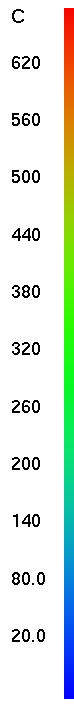
\includegraphics[height=7.0in]{\SMVfigdir/colorbar_20_620}}\\
  \end{tabular}
\end{center}
\caption[Boundary file test of shaded and chopped
contours]{Boundary file test of shaded and chopped contours at
\SI{2}{s}, \SI{10}{s} and \SI{30}{s}. The
upper obstacle is initialized to \SI{600}{\degreeCelsius} and should be red
for the $t\approx\SI{2}{s}$ images. For the chopped contours, the
color near the chop boundary should match the color near
\SI{140}{\degreeCelsius} in the colorbar.}
\label{figboundtest}%
\end{figure}

\clearpage

\section{Iso-surfaces}
An isosurface is a three-dimensional surface that defines constant values of a
dependent variable. Figures \ref{figisotest} and \ref{figisotest2} present
images verifying the display of isosurfaces. A series of temperature isosurfaces
are drawn at \SI{0}{s}, \SI{10}{s} and \SI{30}{s}.  A portion of the interior gas
temperature is initialized to \SI{600}{\degreeCelsius}. This results in the rectangular block
that appears in the first row of images. The first column in
Fig. \ref{figisotest}\ presents the iso-surface using points. The second column
presents the iso-surface using triangulated outlines. The third column presents
the iso-surface using a solid surface. Figure \ref{figisotest2} demonstrates
color customization using the {\tt ISOCOLORS}\ .ini keyword.

\begin{figure}[bph]
\begin{center}
\begin{tabular}{ccc}
 \includegraphics[height=\figheightD]{SCRIPT_FIGURES/plume5c_iso_points_00}&
 \includegraphics[height=\figheightD]{SCRIPT_FIGURES/plume5c_iso_outline_00}&
 \includegraphics[height=\figheightD]{SCRIPT_FIGURES/plume5c_iso_solid_00}\\
 \includegraphics[height=\figheightD]{SCRIPT_FIGURES/plume5c_iso_points_10}&
 \includegraphics[height=\figheightD]{SCRIPT_FIGURES/plume5c_iso_outline_10}&
 \includegraphics[height=\figheightD]{SCRIPT_FIGURES/plume5c_iso_solid_10}\\
 \includegraphics[height=\figheightD]{SCRIPT_FIGURES/plume5c_iso_points_30}&
 \includegraphics[height=\figheightD]{SCRIPT_FIGURES/plume5c_iso_outline_30}&
 \includegraphics[height=\figheightD]{SCRIPT_FIGURES/plume5c_iso_solid_30}\\
 point view&outline view&solid view
  \end{tabular}
\end{center}
 \caption[A test showing an isosurface enclosing a region initialized
 to \SI{600}{\degreeCelsius}]{A test showing an isosurface enclosing a
 region initialized to \SI{600}{\degreeCelsius} at \SI{0}{s}, \SI{10}{s}
 and \SI{30}{s}. The isosurface should surround this region for the $t=\SI{0}{s}$ images.}
\label{figisotest}%
\end{figure}

\begin{figure}[bph]
\begin{center}
\begin{tabular}{cc}
 \includegraphics[height=\figheightD]{SCRIPT_FIGURES/plume5c_iso_solid_30}&
 \includegraphics[height=\figheightD]{SCRIPT_FIGURES/plume5c_iso2_solid_30}\\
 solid view - orange&solid view - blue
  \end{tabular}
\end{center}
 \caption[A test showing isosurfaces colored orange and blue using the
 ISOCOLORS .ini keyword.]{A test showing isosurfaces colored orange and
 blue using the ISOCOLORS .ini keyword at \SI{30}{s}.  The two isosurfaces
 are colored orange and blue using the ISOCOLORS .ini keyword.}
\label{figisotest2}%
\end{figure}

\clearpage

\subsection{Sensitivity Analysis}
\begin{figure}[bph]
\begin{center}
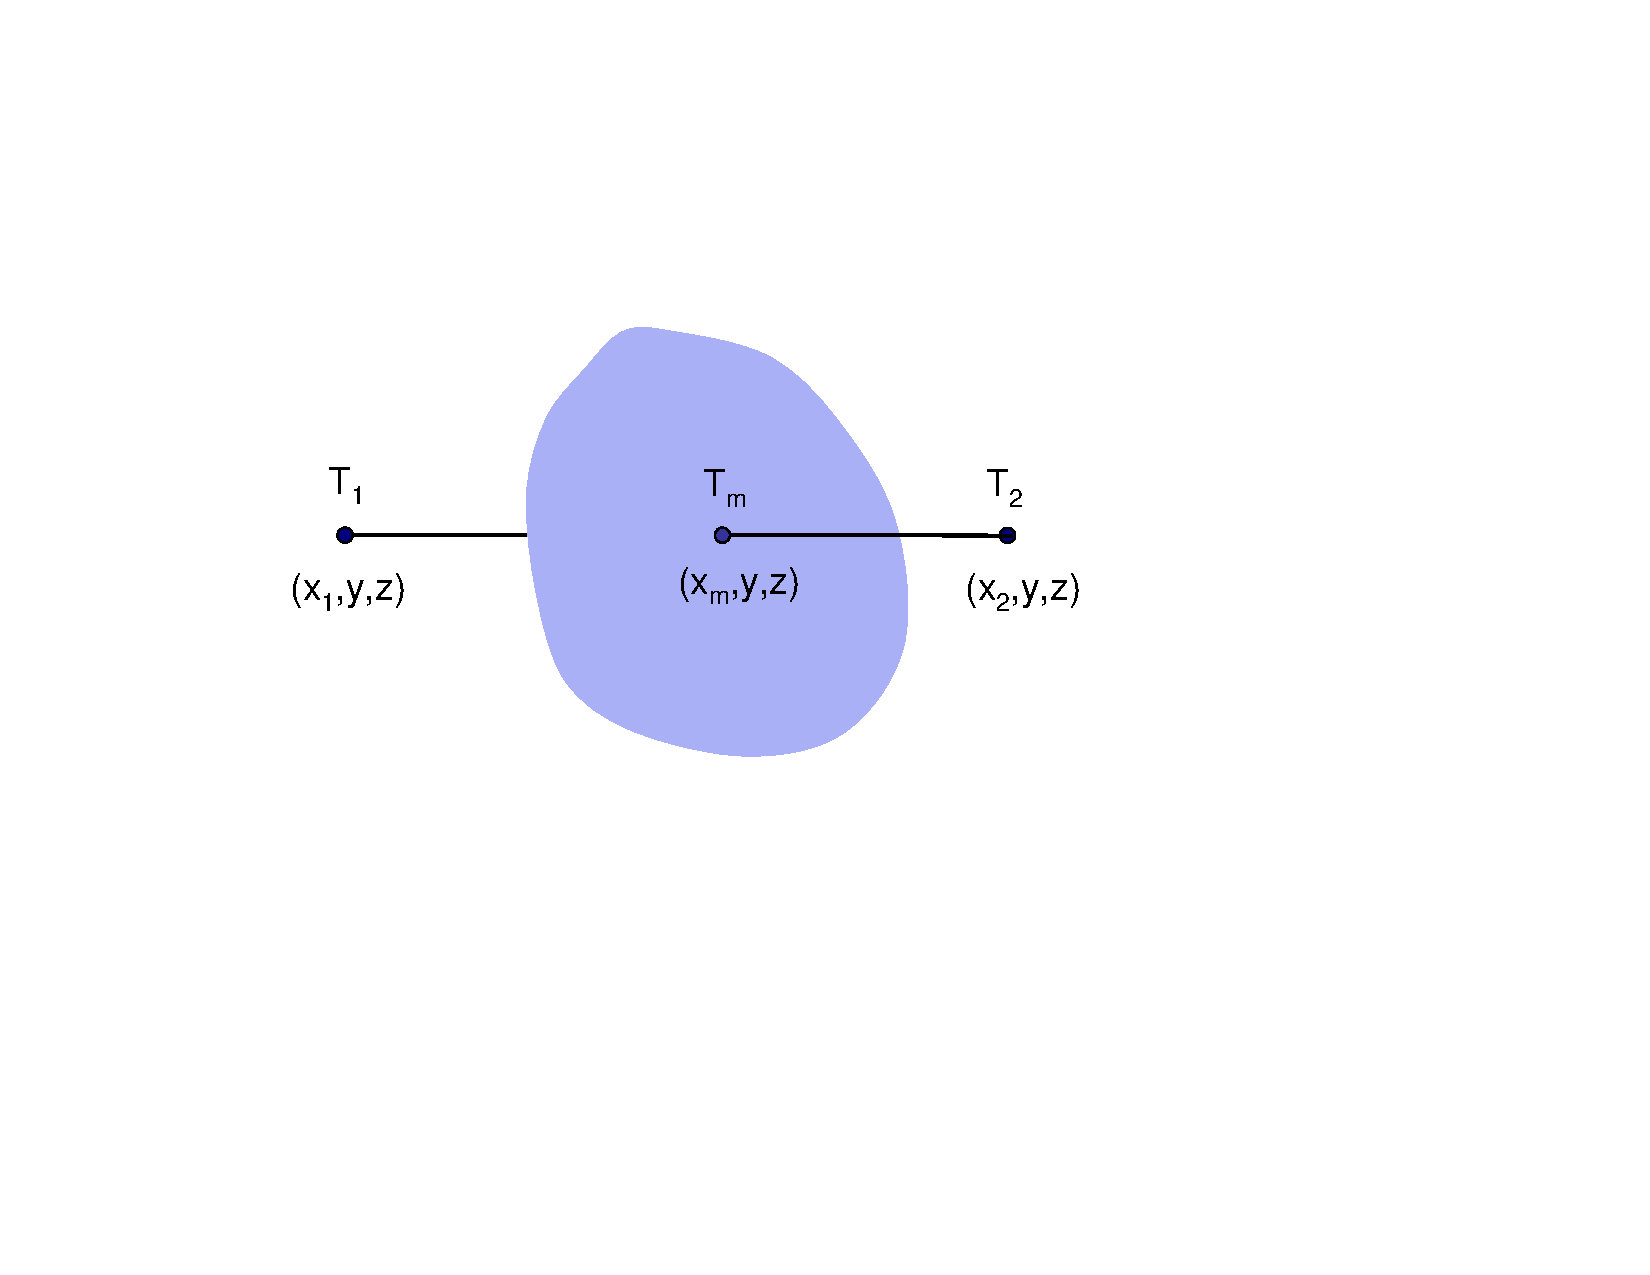
\includegraphics[height=3.0in]{\SMVfigdir/linear_interpolationiso}
\end{center}
 \caption{A portion of an iso-surface defined by $f(x,y,z)=T_m$
 (for some arbitrary function $f$)  crossing a line segment at the point $(x_m,y,z)$.
  }
\label{figisointerpiso}%
\end{figure}

Given that data used to generate an isosurface has uncertainty, an
important question to consider is how sensitive is the isosurface
location to uncertainty in the data used to define it? Figure \ref{figisointerpiso}
shows a portion of an iso-surface, $f(x,y,z)=T_m$, passing through a line segment
at $(x_m,y,z)$. The line segment is defined by endpoints $(x_1,y,z)$ and $(x_2,y,z)$.
The key step in constructing an isosurface is solving an inverse interpolation problem.
That is, determining the location, $(x_m,y,z)$, between two grid nodes,
$(x_1,y,z)$ and $(x_2,y,z)$, where interpolated data takes on a particular value
(the isosurface level, $T_m$, being constructed).

\begin{figure}[bph]
\begin{center}
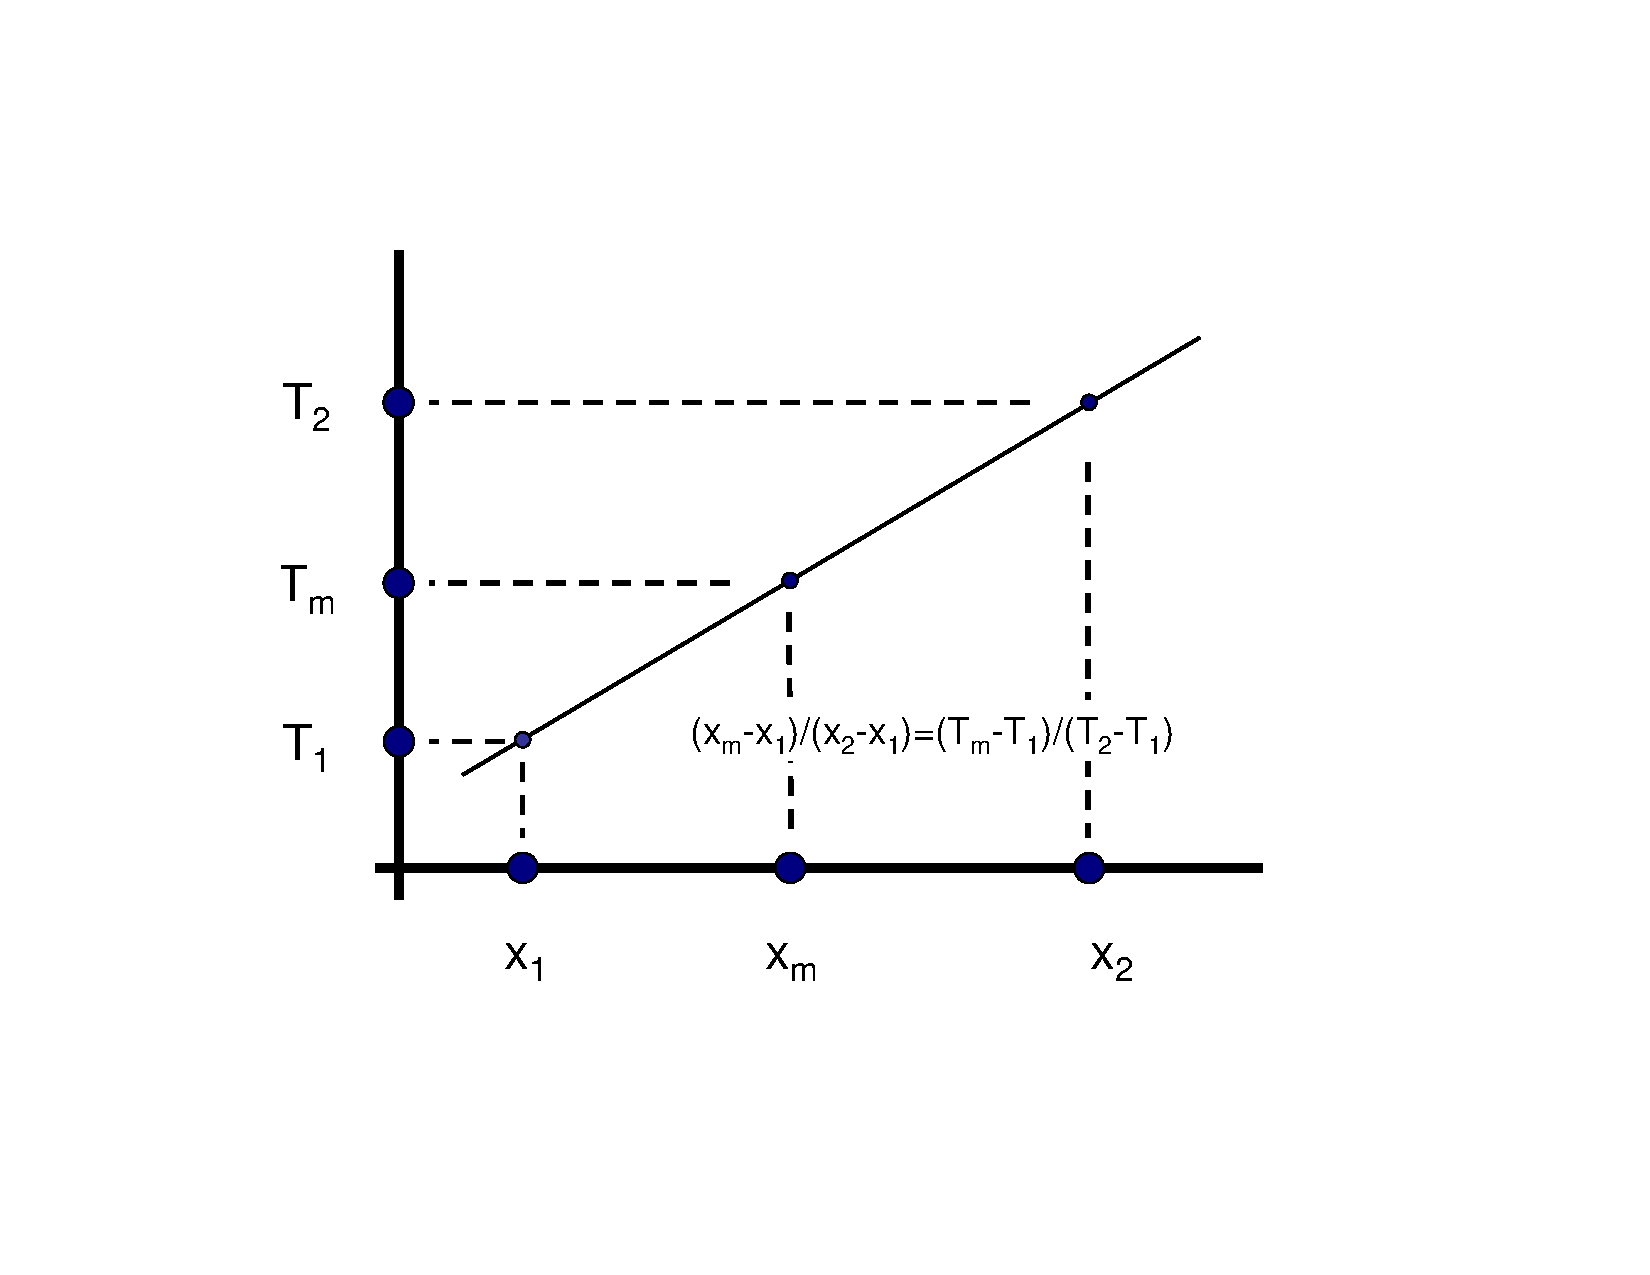
\includegraphics[height=3.0in]{\SMVfigdir/linear_interpolation}
\end{center}
\caption[Diagram setting up an inverse linear interpolation calculation]
{Diagram setting up an inverse linear interpolation calculation.
The dependent data values $T_1$ and $T_2$ are known at locations $x_1$ and $x_2$.
The inverse interpolation problem is to find the location $x_m$ that has value $T_m$.
This is found noting that $(x_m-x_1)/(x_2-x_1)=(T_m-T_1)/(T_2-T_1)$.
 }
\label{figisointerp}%
\end{figure}

Suppose, as illustrated in Fig. \ref{figisointerp}, that $(x_1,y,z)$, $T_1$ and
$(x_2,y,z)$, $T_2$ represent two known data location, data value pairs and
that $T_m$ is also known satisfying $T_1\le T_m \le T_2$.  The inverse
interpolation problem then is to find the location $(x_m,y,z)$ that takes on
the data value $T_m$.  The location $x_m$ is given by

\begin{eqnarray}
x_m=(1-\alpha)x_1+\alpha x_2
\end{eqnarray}
where
\begin{eqnarray}
\alpha=\frac{T_m-T_1}{T_2-T_1}
\end{eqnarray}

\noindent The sensitivity of $x_m$ due to a change $\Delta T_1$ in $T_1$ and to a
change $\Delta T_2$ in $T_2$ is given by
\begin{eqnarray}
\Delta x_m= \pxtone \Delta T_1 + \pxttwo \Delta T_2
\label{eq:sensitivity}
\end{eqnarray}
where
\begin{eqnarray}
\pxtone&=&\pxalpha\palphatone \label{eq:sensfirst}\\
\pxttwo&=&\pxalpha\palphattwo
\end{eqnarray}
and
\begin{eqnarray}
\pxalpha&=&x_2-x_1\\
\palphatone&=&\frac{T_m-T_2}{(T_2-T_1)^2}\\
\palphattwo&=&-\frac{T_m-T_1}{(T_2-T_1)^2}
\label{eq:senslast}
\end{eqnarray}
Equation (\ref{eq:sensitivity}) may be re-written using terms in equations
(\ref{eq:sensfirst}) through (\ref{eq:senslast}) to obtain
\begin{eqnarray}
\frac{\Delta x_m}{x_2-x_1}&=&\frac{T_m-T_2}{(T_2-T_1)^2}\Delta T_1-
\frac{T_m-T_1}{(T_2-T_1)^2}\Delta T_2
=-\left(
(1-\alpha)\frac{\Delta T_1}{T_2-T_1}+
\alpha\frac{\Delta T_2}{T_2-T_1}\right)
\label{eq:sensfinal}
\end{eqnarray}

\noindent Equation (\ref{eq:sensfinal}) relates the relative error of $x_m$ to
the relative errors of $T_1$ and $T_2$ in terms of the interpolation parameter $\alpha$.
The error $\Delta x_m$ may then be bounded to obtain

\begin{eqnarray}
|\Delta x_m|\le
|x_2-x_1|\frac{\max(|\Delta T_1|,|\Delta T_2|)}{|T_2-T_1|}
\end{eqnarray}

\noindent Uncertainty in isosurface location is then proportional to the magnitude
of data uncertainty, $\max(|\Delta T_1|,|\Delta T_2|)$, and inversely proportional
to the data variation, $|T_2-T_1|$.


\clearpage

\section{Particles}

Figure \ref{figparttest} presents images verifying the display of particles and streaks.
Images are drawn at \SI{1}{s}, \SI{10}{s} and \SI{30}{s}. The first column shows particles
while the second and third columns shows streaks with duration \SI{0.5}{s} and \SI{1}{s}.
Streaks are a good way of visualizing motion in a still image (i.e., on paper) since the
streak shows a history of where the particle has been.

\begin{figure}[bph]
\begin{center}
\begin{tabular}{ccc}
 \includegraphics[height=\figheightD]{SCRIPT_FIGURES/plume5c_part_01}&
 \includegraphics[height=\figheightD]{SCRIPT_FIGURES/plume5c_part_streak_01}&
 \includegraphics[height=\figheightD]{SCRIPT_FIGURES/plume5c_part_streak2_01}\\
 \includegraphics[height=\figheightD]{SCRIPT_FIGURES/plume5c_part_10}&
 \includegraphics[height=\figheightD]{SCRIPT_FIGURES/plume5c_part_streak_10}&
 \includegraphics[height=\figheightD]{SCRIPT_FIGURES/plume5c_part_streak2_10}\\
 \includegraphics[height=\figheightD]{SCRIPT_FIGURES/plume5c_part_30}&
 \includegraphics[height=\figheightD]{SCRIPT_FIGURES/plume5c_part_streak_30}&
 \includegraphics[height=\figheightD]{SCRIPT_FIGURES/plume5c_part_streak2_30}\\
 points&\SI{0.5}{s} streaks&\SI{1}{s} streaks\\
  \end{tabular}
\end{center}
 \caption[A test showing particles and particle streaks]{A test showing particles
 and particle streaks at \SI{1}{s}, \SI{10}{s} and \SI{30}{s}}
\label{figparttest}%
\end{figure}


\clearpage

\section{Slices}
Figure \ref{fignodeslicetest} presents images verifying the display of node centered data slices.
Images are drawn at \SI{0}{s}, \SI{10}{s} and \SI{30}{s}. A portion of the interior
gas temperature is initialized to \SI{600}{\degreeCelsius} corresponding to the
red rectangular block appearing in the first row. The first column visualizes
all of the data in the slice.  The second column discards or chops data below
\SI{140}{\degreeCelsius}. Note that the color near the chopped boundary should
match the color in the color bar near \SI{140}{\degreeCelsius}.

Figures \ref{figcellaslicetest} and \ref{figcellbslicetest} present images
verifying the display of cell centered data. Images in Fig. \ref{figcellaslicetest}
are drawn at \SI{0}{s}, \SI{10}{s} and \SI{30}{s}. Images in
Fig. \ref{figcellbslicetest} tests the transfer of data from FDS to Smokeview.

Figure \ref{figslicenodemasktest} and \ref{figslicecellmasktest} presents images verifying that node and cell centered slices
are masked properly when drawn through or near blockages. Images are drawn at \SI{10}{s}.

Figure \ref{figvslicetest} present images verifying the display of vector slices.
Again, vector slice file images are drawn at \SI{0}{s}, \SI{10}{s} and \SI{30}{s}.
The first column draws all vectors while the second column discards or chops vectors
below \SI{140}{\degreeCelsius}.

Figure \ref{figfedslicetest} presents slice file images verifying the computation
of fractional effective dose (FED).  FED is a measure of human incapacitation or
hazard due to combustion gases\cite{SFPE:Purser}. Images are drawn at \SI{30}{s},
\SI{60}{s} and \SI{120}{s} and \SI{240}{s}. The FED is computed using three data slices with concentration of $1000~\mathrm{ppm}$ for $\mathrm{CO}$ and volume fractions of 0.02 and 0.07 for $\mathrm{CO_2}$ and $\mathrm{O_2}$ respectively. These values result in FED values of 1.5 at \SI{30}{s}, 3.0 at \SI{60}{s}, 6.0 at \SI{120}{s} and 12.0 at \SI{240}{s}.

Figure \ref{figgslicetest} presents images of 3D slices oriented in two different
ways. Images are drawn at \SI{0}{s}, \SI{10}{s} and \SI{30}{s}.
Figure \ref{figvgslicetest} presents images of 3D vector slices oriented in two different
ways. Images are drawn at \SI{0}{s}, \SI{10}{s} and \SI{30}{s}.

Figure \ref{figdiffslicetest} presents images from data differenced by Smokediff.
Smokediff computed the difference between two similar FDS cases and generated slice
files. Difference contours from these slice files are displayed at \SI{0}{s},
\SI{10}{s} and \SI{15}{s}.

\begin{figure}[bph]
\begin{center}
\begin{tabular}{cccp{1.0in}}
 \includegraphics[height=\figheightE]{SCRIPT_FIGURES/plume5c_slice_00}&
 \includegraphics[height=\figheightE]{SCRIPT_FIGURES/plume5c_slice_chop_00}\\

 \includegraphics[height=\figheightE]{SCRIPT_FIGURES/plume5c_slice_10}&
 \includegraphics[height=\figheightE]{SCRIPT_FIGURES/plume5c_slice_chop_10}\\

 \includegraphics[height=\figheightE]{SCRIPT_FIGURES/plume5c_slice_30}&
 \includegraphics[height=\figheightE]{SCRIPT_FIGURES/plume5c_slice_chop_30}\\

 node centered data&node centered chopped data\\
&&\raisebox{0.5in}[0pt]{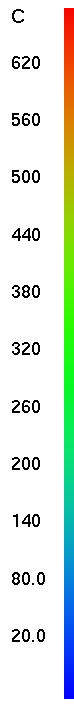
\includegraphics[height=7.5in]{\SMVfigdir/colorbar_20_620}}\\
 \end{tabular}
\end{center}
 \caption[A test showing shaded and chopped contours of node centered slice
 file data]{A test showing shaded and chopped contours of node centered slice
 file data at \SI{0}{s}, \SI{10}{s} and \SI{30}{s}.  A portion of the interior
 gas temperature is initialized to \SI{600}{\degreeCelsius}.  The slice file
 in this region should be red for the $t=\SI{0}{s}$ images.  For the chopped
 contours, the color near the chop boundary should match the color near
 \SI{140}{\degreeCelsius} in the colorbar.}
\label{fignodeslicetest}%
\end{figure}

\begin{figure}[bph]
\begin{center}
\begin{tabular}{cccp{1.0in}}
 \includegraphics[height=\figheightE]{SCRIPT_FIGURES/plume5c_slice_cell_00}&
 \includegraphics[height=\figheightE]{SCRIPT_FIGURES/plume5c_slice_cellchop_00}\\

 \includegraphics[height=\figheightE]{SCRIPT_FIGURES/plume5c_slice_cell_10}&
 \includegraphics[height=\figheightE]{SCRIPT_FIGURES/plume5c_slice_cellchop_10}\\

 \includegraphics[height=\figheightE]{SCRIPT_FIGURES/plume5c_slice_cell_30}&
 \includegraphics[height=\figheightE]{SCRIPT_FIGURES/plume5c_slice_cellchop_30}\\

 cell centered data&cell centered chopped data\\
 &&\raisebox{0.5in}[0pt]{\includegraphics[height=7.5in]{\SMVfigdir/colorbar_20_620}}\\
 \end{tabular}
\end{center}
 \caption[A test showing shaded and chopped contours of cell centered slice file
 data]{A test showing shaded and chopped contours of cell centered slice file data
 at \SI{0}{s}, \SI{10}{s} and \SI{30}{s}.  A portion of the interior gas temperature
 is initialized to \SI{600}{\degreeCelsius}.  The slice file in this region should
 be red for the $t=\SI{0}{s}$ images.  For the chopped contours, the color near the
 chop boundary should match the color near \SI{140}{\degreeCelsius} in the colorbar.}
\label{figcellaslicetest}%
\end{figure}

\begin{figure}[bph]
\begin{center}
\begin{tabular}{cc}

 \includegraphics[width=2.55in]{SCRIPT_FIGURES/cell_test_z}&
 \includegraphics[width=2.75in]{SCRIPT_FIGURES/cell_test_3D}\\

 a) plan view (top slice)&
 b) 3D view\\
 \vspace{0.01in}\\
 \includegraphics[width=2.55in]{SCRIPT_FIGURES/cell_test_y}&
 \includegraphics[width=3.4in]{SCRIPT_FIGURES/cell_test_x}\\
  c) elevation view (front slice)&
  d) side view (right slice)\\
\end{tabular}
\end{center}
 \caption[A test to demonstrate that cell centered slice file  data is transferred
 from FDS to Smokeview properly.]{A test to demonstrate that cell centered slice file
 data is transferred to Smokeview properly.  Cell values are initialized in
 FDS to $100*i + 10*j + k$ where $1\le i \le 3$, $1\le j \le 4$ and $1\le k \le 5$.
 Cell values displayed should match the $(i,j,k)$ grid cell indices.  The three plots
 in the 3D view correspond to the plan, elevation and side view plots.}
\label{figcellbslicetest}%
\end{figure}

\begin{figure}[bph]
\begin{center}
\begin{tabular}{cc}
 \includegraphics[width=2.25in]{SCRIPT_FIGURES/slicemask_node1}&
 \includegraphics[width=2.25in]{SCRIPT_FIGURES/slicemask_node2}\\
 below&below on boundary\\
 \includegraphics[width=2.25in]{SCRIPT_FIGURES/slicemask_node3}&
  \includegraphics[width=2.25in]{SCRIPT_FIGURES/slicemask_node4}\\
above on boundary&above
\end{tabular}
\end{center}
 \caption[A test to demonstrate that node centered slice files are masked properly.]
 {A test to demonstrate that node centered slice files are masked properly when drawn through or near blockages.}
\label{figslicenodemasktest}%
\end{figure}

\begin{figure}[bph]
\begin{center}
\begin{tabular}{ccc}
 \includegraphics[width=2.250in]{SCRIPT_FIGURES/slicemask_cell1}&
 \includegraphics[width=2.25in]{SCRIPT_FIGURES/slicemask_cell2}&
 \includegraphics[width=2.25in]{SCRIPT_FIGURES/slicemask_cell3}\\
 below&through&above
\end{tabular}
\end{center}
 \caption[A test to demonstrate that cell centered slice files are masked properly.]
 {A test to demonstrate that cell centered slice files are masked properly when drawn through or near blockages.}
\label{figslicecellmasktest}%
\end{figure}

\begin{figure}[bph]
\begin{center}
\begin{tabular}{ccl}
 \includegraphics[height=\figheightE]{SCRIPT_FIGURES/plume5c_vslice_00}&
 \includegraphics[height=\figheightE]{SCRIPT_FIGURES/plume5c_vslicechop_00}\\
 \includegraphics[height=\figheightE]{SCRIPT_FIGURES/plume5c_vslice_10}&
 \includegraphics[height=\figheightE]{SCRIPT_FIGURES/plume5c_vslicechop_10}\\
 \includegraphics[height=\figheightE]{SCRIPT_FIGURES/plume5c_vslice_30}&
 \includegraphics[height=\figheightE]{SCRIPT_FIGURES/plume5c_vslicechop_30}\\
 &data chopped below \SI{140}{\degreeCelsius}\\
 &&\raisebox{0.5in}[0pt]{\includegraphics[height=7.5in]{\SMVfigdir/colorbar_20_620}}\\

 \end{tabular}
\end{center}
 \caption[A test showing vector slice file data] {A test showing vector slice file data
 at \SI{1}{s}, \SI{10}{s} and \SI{30}{s}. A portion of the interior gas temperature
 is initialized to \SI{600}{\degreeCelsius}.  The vectors in this region should be
 red for the $t=\SI{0}{s}$ images. For the chopped contours, the color near the chop
 boundary should match the color near \SI{140}{\degreeCelsius} in the colorbar.}
\label{figvslicetest}%
\end{figure}

\begin{figure}[bph]
\begin{center}
\begin{tabular}{ccp{1.0in}}
 \includegraphics[height=\figheightE]{SCRIPT_FIGURES/fed_test_030}&
 \includegraphics[height=\figheightE]{SCRIPT_FIGURES/fed_test_060}\\
SI{30}{s}, FED=0.29&\SI{60}{s}, FED=0.59\\
 \includegraphics[height=\figheightE]{SCRIPT_FIGURES/fed_test_120}&
 \includegraphics[height=\figheightE]{SCRIPT_FIGURES/fed_test_360}\\
\SI{120}{s}, FED=1.2&3\SI{60}{s}, FED=3.5\\
&&\raisebox{0.25in}[0pt]{\includegraphics[height=5.5in]{\SMVfigdir/colorbar_fed}}
 \end{tabular}
\end{center}
 \caption[A test showing cell centered FED slice file data]{A test showing cell
 centered FED slice file data.  These contours were generated using $\mathrm{CO}$,
 $\mathrm{CO_2}$ and $\mathrm{O_2}$ data slices. }
\label{figfedslicetest}%
\end{figure}

\begin{figure}[bph]
\begin{center}
\begin{tabular}{cccp{1.0in}}
 \includegraphics[height=\figheightE]{SCRIPT_FIGURES/plume5c_gslice_00}&
 \includegraphics[height=\figheightE]{SCRIPT_FIGURES/plume5c_gslice2_00}\\

 \includegraphics[height=\figheightE]{SCRIPT_FIGURES/plume5c_gslice_10}&
 \includegraphics[height=\figheightE]{SCRIPT_FIGURES/plume5c_gslice2_10}\\

 \includegraphics[height=\figheightE]{SCRIPT_FIGURES/plume5c_gslice_30}&
 \includegraphics[height=\figheightE]{SCRIPT_FIGURES/plume5c_gslice2_30}\\

 general orientation&second orientation\\
 &&\raisebox{0.5in}[0pt]{\includegraphics[height=7.5in]{\SMVfigdir/colorbar_20_620}}\\
 \end{tabular}
\end{center}
 \caption[A test showing arbitrarily oriented slice file planes generated from
 3D slice files]{A test showing arbitrarily oriented slice file planes generated
 from 3D slice files at \SI{0}{s}, \SI{10}{s} and \SI{30}{s}.  Two orientations are
 shown at three time steps. }
\label{figgslicetest}%
\end{figure}


\begin{figure}[bph]
\begin{center}
\begin{tabular}{cccp{1.0in}}
 \includegraphics[height=\figheightE]{SCRIPT_FIGURES/plume5c_vgslice_00}&
 \includegraphics[height=\figheightE]{SCRIPT_FIGURES/plume5c_vgslice2_00}\\

 \includegraphics[height=\figheightE]{SCRIPT_FIGURES/plume5c_vgslice_10}&
 \includegraphics[height=\figheightE]{SCRIPT_FIGURES/plume5c_vgslice2_10}\\

 \includegraphics[height=\figheightE]{SCRIPT_FIGURES/plume5c_vgslice_30}&
 \includegraphics[height=\figheightE]{SCRIPT_FIGURES/plume5c_vgslice2_30}\\

 general orientation&second orientation\\
 &&\raisebox{0.5in}[0pt]{\includegraphics[height=7.5in]{\SMVfigdir/colorbar_20_620}}\\
 \end{tabular}
\end{center}
 \caption[A test showing arbitrarily oriented vector slice file planes generated from
 3D slice files]{A test showing arbitrarily oriented vector slice file planes generated
 from 3D slice files at \SI{0}{s}, \SI{10}{s} and \SI{30}{s}.  Two orientations are
 shown at three time steps. }
\label{figvgslicetest}%
\end{figure}

\begin{figure}[bph]
\begin{center}
\begin{tabular}{cp{1.0in}}
 \includegraphics[height=\figheightE]{SCRIPT_FIGURES/plume5c_diff_slice_00}\\
 \includegraphics[height=\figheightE]{SCRIPT_FIGURES/plume5c_diff_slice_10}\\
 \includegraphics[height=\figheightE]{SCRIPT_FIGURES/plume5c_diff_slice_30}\\
&\raisebox{0.5in}[0pt]{\includegraphics[height=7.5in]{\SMVfigdir/colorbar_tempdiff}}\\
 \end{tabular}
\end{center}
 \caption[A test showing slice contours generated by differencing two cases with
 Smokediff]{A test showing slice contours generated by differencing
 two cases with Smokediff  at \SI{0}{s}, \SI{10}{s} and \SI{30}{s}.}
\label{figdiffslicetest}%
\end{figure}


\clearpage

\section{3D Smoke}

Figure \ref{figsmoketest} presents images verifying the display of 3D smoke and fire
(heat release rate per unit volume or HRRPUV). A series of 3D smoke images are drawn
at \SI{1}{s}, \SI{10}{s} and \SI{30}{s}.  The images contain semi-transparent slices
derived from both soot density and HRRPUV data.

\begin{figure}[bph]
\begin{center}
\begin{tabular}{ccc}
 \includegraphics[height=\figheightD]{SCRIPT_FIGURES/plume5c_smoke_01}&
 \includegraphics[height=\figheightD]{SCRIPT_FIGURES/plume5c_smoke_10}&
 \includegraphics[height=\figheightD]{SCRIPT_FIGURES/plume5c_smoke_30}
\end{tabular}
\end{center}
 \caption{A test showing 3D smoke drawn at \SI{1}{s}, \SI{10}{s} and \SI{30}{s}}
\label{figsmoketest}%
\end{figure}

\clearpage

\section{Plot3D}

Figure \ref{figPLOT3Dtest} presents images verifying the display of PLOT3D contours.
Three types of contours are available for visualizing PLOT3D data: stepped,
continuous and narrow band.  This figure shows stepped and continuous contours.
Figure \ref{figPLOT3Dtestvalue} shows stepped contours in at four positions along the y axis.
Figure \ref{figPLOT3Dtestline} shows narrow band contours at four positions front to back.
Figure \ref{figPLOT3Dtestvector} shows velocity vectors at the same four positions as in
Figure \ref{figPLOT3Dtestvalue}.
Figure \ref{figPLOT3Dtestiso} shows PLOT3D iso-surfaces for \SI{50}{\degreeCelsius},
\SI{230}{\degreeCelsius}, \SI{410}{\degreeCelsius} and \SI{590}{\degreeCelsius}.

\begin{figure}[bph]
\begin{center}
\begin{tabular}{cc}
 \includegraphics[height=\figheightD]{SCRIPT_FIGURES/plume5c_plot3d_step}&
 \includegraphics[height=\figheightD]{SCRIPT_FIGURES/plume5c_plot3d_shaded}\\
 step contours&
 continuous contours
 \end{tabular}
\end{center}
 \caption{A test showing PLOT3D stepped and continuous temperature contours.}
\label{figPLOT3Dtest}%
\end{figure}

\begin{figure}[bph]
\begin{center}
\begin{tabular}{cc}
 \includegraphics[height=\figheightH]{SCRIPT_FIGURES/plume5c_plot3d_y1}&
 \includegraphics[height=\figheightH]{SCRIPT_FIGURES/plume5c_plot3d_y2}\\
 \includegraphics[height=\figheightH]{SCRIPT_FIGURES/plume5c_plot3d_y3}&
 \includegraphics[height=\figheightH]{SCRIPT_FIGURES/plume5c_plot3d_y4}\\
 \end{tabular}
\end{center}
 \caption{A test showing PLOT3D stepped contours at four positions along the y axis.}
\label{figPLOT3Dtestvalue}%
\end{figure}

\begin{figure}[bph]
\begin{center}
\begin{tabular}{cc}
 \includegraphics[height=\figheightH]{SCRIPT_FIGURES/plume5c_plot3d_l1}&
 \includegraphics[height=\figheightH]{SCRIPT_FIGURES/plume5c_plot3d_l2}\\
 \includegraphics[height=\figheightH]{SCRIPT_FIGURES/plume5c_plot3d_l3}&
 \includegraphics[height=\figheightH]{SCRIPT_FIGURES/plume5c_plot3d_l4}\\
 \end{tabular}
\end{center}
 \caption{A test showing PLOT3D narrow band contours at four positions along the y axis.}
\label{figPLOT3Dtestline}%
\end{figure}

\begin{figure}[bph]
\begin{center}
\begin{tabular}{cc}
 \includegraphics[height=\figheightH]{SCRIPT_FIGURES/plume5c_plot3d_v1}&
 \includegraphics[height=\figheightH]{SCRIPT_FIGURES/plume5c_plot3d_v2}\\
 \includegraphics[height=\figheightH]{SCRIPT_FIGURES/plume5c_plot3d_v3}&
 \includegraphics[height=\figheightH]{SCRIPT_FIGURES/plume5c_plot3d_v4}\\
 \end{tabular}
\end{center}
 \caption{A test showing PLOT3D vectors shaded by temperature at four positions
 along the y axis.}
\label{figPLOT3Dtestvector}%
\end{figure}

\begin{figure}[bph]
\begin{center}
\begin{tabular}{ccl}
 \includegraphics[height=\figheightH]{SCRIPT_FIGURES/plume5c_plot3d_i1}&
 \includegraphics[height=\figheightH]{SCRIPT_FIGURES/plume5c_plot3d_i2}\\
 \SI{50}{\degreeCelsius}&\SI{230}{\degreeCelsius}\\
  \includegraphics[height=\figheightH]{SCRIPT_FIGURES/plume5c_plot3d_i3}&
 \includegraphics[height=\figheightH]{SCRIPT_FIGURES/plume5c_plot3d_i4}\\
 \SI{410}{\degreeCelsius}&\SI{590}{\degreeCelsius}\\
&&\raisebox{0.5in}[0pt]{\includegraphics[height=7.5in]{\SMVfigdir/colorbar_050_590_plot3d_iso}}\\
 \end{tabular}
\end{center}
 \caption{A test showing PLOT3D iso-surfaces for \SI{50}{\degreeCelsius},
 \SI{230}{\degreeCelsius}, \SI{410}{\degreeCelsius} and \SI{590}{\degreeCelsius}.}
\label{figPLOT3Dtestiso}%
\end{figure}

\chapter{Smoke Visualization Tests}

Correct smoke visualization requires that smoke flow be both computed and drawn correctly.
The FDS Verification Guide~\cite{FDS_Verification_Guide} addresses computation in terms of
soot/smoke production, transport, etc. A verification of how smoke is drawn is addressed in
this chapter. More precisely, given a known density and distribution of soot, does the smoke
drawn by Smokeview match how {\em theory}\ predicts it should appear.  Presently, the main
interest is in how smoke obscures objects in the background.  Visualization effects due to
light scattering are not modeled.

The smoke drawing verification problem is split into two steps. The first step,
documented in Section \ref{sect:record_smoke}, is to verify that Smokeview can record
the correct grey level of smoke as it is drawn on the screen. This step is necessary
because screen colors, in this case the smoke obscuration levels to be verified, are
not directly accessible to Smokeview. They must be retrieved from the video card
buffers. The second step, documented in Section \ref{sect:verify_smoke}, is to
verify that Smokeview can draw the correct shade of grey given a known soot density level
within the scene.
\section{Recording Smoke Levels}
\label{sect:record_smoke}

Smokeview does not have direct access to colors drawn on the screen.
Smokeview passes vertex colors to the video driver.
The video driver then interpolates colors within these vertices.
Smokeview must then `read' them back in after they are drawn.
A further complication is that smoke is drawn in Smokeview using a physical coordinate system.
The smoke opacity levels are retrieved using the screen coordinate system, ie.
at particular pixel locations.
It is this transformation process, from physical to screen coordinates,
that is verified in this step.

In the case of 3D smoke visualization, these colors represent smoke opacity levels.
To obtain these levels and thereby verifying that they are correct,
Smokeview makes use of a special sensor or device named {\em smokesensor}\
which Smokeview uses to obtain color values at the sensor location.
This device behaves like other FDS devices but has the additional
property that when used by Smokeview, it displays the grey level as viewed by the observer.
This grey level is displayed as a number between 0 and 255.

The user places a device of type {\tt smoke\_sensor}\ at a particular $(x, y, z)$ location using statements such as

{\small
\begin{verbatim}
&PROP ID='smoketest' SMOKEVIEW_ID='smokesensor' /
&DEVC XYZ=1.8,0.55,2.00, QUANTITY='VISIBILITY', ID='vis1' PROP_ID='smoketest' /
\end{verbatim}
}

Smokeview displays the sensor as a white disk with color (255,255,255) at location $(1.8,0.55,2.00)$
always oriented towards the observer. When drawing smoke that resides between
the sensor and the observer (your eye), the smoke sensor is partially obscured by the smoke.
Smokeview then alters the smoke sensor color according to how much and how thick the
intervening smoke is.  It does this by blending each smoke plane, one plane at a time, using
the color and opacity levels of that plane. The grey level is simply Smokeview's
computation of the integrated {\em smoke thickness}\ along a path between the sensor
location and the eye.  The colors displayed are the result of computations performed by the
video card using OpenGL, the graphics library used by Smokeview to visualize FDS scenarios.

Figure \ref{figsmokesensor} illustrates an initial test of this process.
It verifies that Smokeview can transform the sensor location from physical
or FDS coordinates to screen coordinates (pixel locations) and further
can correctly record the grey level at those screen coordinates even when
surrounded by other objects with different colors.
In this case, the smoke sensor is white and there is no intervening smoke.
The background is a neutral grey with grey level of 128.
The value displayed over the sensor then should always be 255 not 128 no matter
how the scene is oriented.
If Smokeview made an error determining the sensor screen coordinates the grey level
displayed would be 128 (grey level of the adjacent grey background) not 255
(grey level of the sensor).

\begin{figure}[bph]
\begin{center}
 \centering
\begin{tabular}{cc}
\includegraphics[width=3.0in]{SCRIPT_FIGURES/smoke_sensor}&
 \end{tabular}
\end{center}
\caption[A test verifying that the Smokeview smoke\_sensor object is working properly]
{A test verifying that Smokeview can correctly transform the physical $(x,y,z)$
location of the smoke\_sensor object to its equivalent screen coordinates where
the underlying smoke obscuration level is retrieved. A small white (255,255,255)
smoke\_sensor appears in front of a grey (128,128,128) obstacle. The value displayed
should be 255,  the value recorded by Smokeview.  If the physical to screen
transformation is performed incorrectly a value of 128 will be displayed (since it
will pick up a color elsewhere).
}
\label{figsmokesensor}%
\end{figure}

\section{Verifying Smoke Transparency}
\label{sect:verify_smoke}

Smoke transparency is verified by setting up a scenario with uniform smoke density and
comparing observed transparency
levels with transparency levels calculated using a scaled form of Bouguer's Law,

\begin{equation}
\tau = 255 \; \exp(-K_m \, S \, \Delta x),
\label{eq:Beers}
\end{equation}

\noindent where $\tau$ is the
transparency\footnote{Smokeview, as all do OpenGL programs, draw objects in terms of opaqueness the inverse of transparency, $\alpha = 255 - \tau$.}
scaled from 0 (completely opaque) to 255 (completely transparent), $K_m=\SI{8700}{m^2/kg}$~\cite{Mulholland:F+M} is the mass extinction coefficient, $S$ is the soot density and $\Delta x$ is the path length through which transparency is observed. This equation is then used to place blockages so that known transparency levels result.

The soot density required to obtain a transparency of $\tau=128$ for a path length of $\Delta x=\SI{1.0}{m}$ is found by solving Eq.~(\ref{eq:Beers}) for $S$ to obtain

\begin{equation}
S=-\frac{\ln(\tau/255)}{K_m\Delta x} = 7.922 \times 10^{-5}\,{\rm kg/m}^3
\label{eq:soot}
\end{equation}

\noindent This soot density is converted to a soot mass fraction for use in the FDS input file by dividing by the air density $\rho_{\rm air}\approx \SI{1.196}{kg/m^3}$ to obtain

\begin{equation}
Y_{\rm soot}=S/\rho_{\rm air}=6.624 \times 10^{-5}\,{\rm kg/kg}~.
\end{equation}

\noindent For this value of soot density, Eq.~(\ref{eq:soot}) can used to simplify Eq. (\ref{eq:Beers}) after noting that $128/255=\exp(-K_mS)$ to obtain

\begin{equation}
\tau = 255 \; \left(\frac{128}{255}\right)^{\Delta x}
\label{eq:Beers2}
\end{equation}

\noindent which is then used to find transparencies for path lengths of
$\Delta x=\SI{5}{m}$, $\SI{4}{m}$, $\SI{3}{m}$, $\SI{2}{m}$, $\SI{1}{m}$, $\SI{0.5}{m}$
which are approximately $\tau=8$, 16, 32, 64, 128 and 181 .
These transparency levels can then be compared to observed levels when viewing the case.

\begin{figure}[bph]
\begin{center}
 \centering
\begin{tabular}{c}
 \includegraphics[height=4.0in]{SCRIPT_FIGURES/smoke_test_side}
 \end{tabular}
\end{center}
 \caption[Side view of the numerical smoke test compartment.]{Side view of the numerical
 smoke test compartment.  Blockages are placed at \SI{0.5}{m}, \SI{1}{m}, \SI{2}{m},
 \SI{3}{m}, \SI{4}{m} , \SI{5}{m} from the front of the domain to make the scaled transparency levels have values
 181, 128, 64, 32, 16 and 8 respectively.}
\label{figsmoketestgeom}%
\end{figure}

Figure~\ref{figsmoketest2} shows quantitative tests of the smoke transparency
calculation performed in Smokeview for three grid resolutions.
This figure also gives the expected transparency levels based upon the specified soot densities, mass extinction coefficient and path lengths.  The smoke visualization algorithm is verified then if the expected shades of grey match the corresponding predicted shades of grey.  Each shaded rectangle is accompanied by a numerical value that can also be used to judge whether the visualization is verified.

The numbers displayed in the upper row of the \SI{0.125}{m}, \SI{0.25}{m} and \SI{0.50}{m} resolution images in Fig. \ref{figsmoketest2} represent the computed smoke transparency levels (ranging from 0 to 255).  These numbers may be verified by using a
program that reports pixel values of this
rectangular region.  The numbers are verified when they match the reported pixel
values. The numbers displayed in the lower row of both resolution images represent the expected transparency levels.

\begin{figure}[bph]
\begin{center}
 \centering
\begin{tabular}{c}
 \includegraphics[width=5.00in]{SCRIPT_FIGURES/smoke_test_all}\\
0.125 m grid\\ \\
 \includegraphics[width=5.00in]{SCRIPT_FIGURES/smoke_test2_all} \\
0.25 m grid\\ \\
 \includegraphics[width=5.00in]{SCRIPT_FIGURES/smoke_test3_all}\\
0.5 m grid\\ \\
 \end{tabular}
\end{center}
 \caption[A test verifying smoke transparency for three grid resolutions.]{A test verifying
 smoke transparency for three grid resolutions.  This test fills the space with a uniform distribution of soot so that blockages
 placed 0.5, 1.0, 2.0, 3.0, 4.0 and 5.0 m from the front of the domain result in
 in grey levels of  181, 128, 64, 32, 16 and 8 respectively.
 }
\label{figsmoketest2}%
\end{figure}


\chapter{WUI Test Cases}
\newcommand{\npage}{}
\newcommand{\chap}{chapter}
This \chap\ presents techniques added to Smokeview~\cite{Smokeview_Tech_Guide} applicable
for visualizing WUI (wildland urban interface) and wild fire scenarios.  Two techniques
involve 1) visualizing changing terrain using satellite images with modeling results
overlayed and 2) making use of geometric objects for representing modeling elements
such as trees or building structures. These two techniques use data generated by fire
models such as FDS~\cite{FDS_Tech_Guide}.
A third technique involves visualizing experimentally derived data rather than modeling
data.  Wind sensor data is visualized using flow vectors along with visual indicators
of data uncertainty. Smokeview images are displayed in the following figures to
illustrate these techniques.

Figure \ref{figlevelset} presents contours of a level set computation.
The level set contours are drawn on a sloped terrain. These level set
contours represent a fire line. A fire line is used with wildland fire
simulations as an efficient method for visualizing the motion of a fire
across the simulation. A fire line in the context of Smokeview is just a
special case of a temperature slice contour.  The thin red line represents
the location where burning is currently taking place.  The grey region
represents where burning has occurred and the green region represents
where burning has not occurred. Level sets are used to quickly (relative
to a complete computational fluid dynamic calculation ) model fire spread
and fire line locations. In this particular case, images are drawn at
\SI{30}{s}, \SI{60}{s}, \SI{90}{s} and \SI{120}{s}. The test verifies
that the level set slices follow the sloped terrain. Figure \ref{figterrain2}
and \ref{figterrain3} also present images of level set contours.
These contour slices are drawn along with a satellite image of the region being modeled.

\begin{figure}[bph]
\begin{center}
\begin{tabular}{cc}
 \includegraphics[height=\figheightE]{SCRIPT_FIGURES/levelset_30}&
 \includegraphics[height=\figheightE]{SCRIPT_FIGURES/levelset_60}\\
 \SI{30}{s}&\SI{60}{s}\\

 \includegraphics[height=\figheightE]{SCRIPT_FIGURES/levelset_90}&
 \includegraphics[height=\figheightE]{SCRIPT_FIGURES/levelset_120}\\
 \SI{90}{s}&\SI{120}{s}

 \end{tabular}
\end{center}
 \caption[A test showing level set slices drawn along a sloped terrain]
 {A test showing level set slices drawn along a sloped terrain at \SI{30}{s},
 \SI{60}{s}, \SI{90}{s} and \SI{120}{s}. The test verifies that level set
 slices follow the sloped terrain. The thin red line represents where
 burning is currently taking place. The grey and green regions represent
 where burning has and has not occurred respectively.}
\label{figlevelset}%
\end{figure}

\begin{figure}[bph]
\begin{center}
\begin{tabular}{cc}
 \includegraphics[height=2.5in]{SCRIPT_FIGURES/BT10m_2x2km_LS_0000}&
 \includegraphics[height=2.5in]{SCRIPT_FIGURES/BT10m_2x2km_LS_0300}\\
 \SI{0}{s}&\SI{300}{s}\\

 \includegraphics[height=2.5in]{SCRIPT_FIGURES/BT10m_2x2km_LS_0600}&
 \includegraphics[height=2.5in]{SCRIPT_FIGURES/BT10m_2x2km_LS_0900}\\
 \SI{600}{s}&\SI{900}{s}\\

 \includegraphics[height=2.5in]{SCRIPT_FIGURES/BT10m_2x2km_LS_1200}&
 \includegraphics[height=2.5in]{SCRIPT_FIGURES/BT10m_2x2km_LS_1500}\\
 \SI{1200}{s}&\SI{1500}{s}\\
 \end{tabular}
\end{center}
 \caption[A test showing a fire line slice drawn along a sloped and textured terrain]
 {A test showing a fire line slice drawn along a sloped and textured terrain
 at \SI{0}{s}, \SI{300}{s}, \SI{600}{s}, \SI{900}{s}, \SI{1200}{s}, and
 \SI{1500}{s} of simulated time. The test verifies that the level set
 slices follow the sloped terrain.}
\label{figterrain2}%
\end{figure}

\begin{figure}[bph]
\begin{center}
\begin{tabular}{c}
 \includegraphics[height=5.5in]{SCRIPT_FIGURES/BT10m_2x2km_LS_1800}\\
 \end{tabular}
\end{center}
 \caption{A test showing a fire line slice drawn along a sloped and textured
 terrain at \SI{1800}{s} simulated time.}
\label{figterrain3}%
\end{figure}

\npage

Figure \ref{figterrain} presents images of temperature contours drawn on a
terrain geometry. The scenario consists of a small hill parallel to the
vertical axis of the scene. Images are drawn at \SI{15}{s}, \SI{30}{s},
\SI{45}{s} and \SI{60}{s}. The test verifies that temperature contours
follow the sloped terrain and that the red blockage (a non-terrain
blockage representing a structure) is drawn correctly along with the terrain.

\begin{figure}[bph]
\begin{center}
\begin{tabular}{cc}
 \includegraphics[height=\figheightE]{SCRIPT_FIGURES/hill_structure_015}&
 \includegraphics[height=\figheightE]{SCRIPT_FIGURES/hill_structure_030}\\
 \SI{15}{s}&\SI{30}{s}\\

 \includegraphics[height=\figheightE]{SCRIPT_FIGURES/hill_structure_045}&
 \includegraphics[height=\figheightE]{SCRIPT_FIGURES/hill_structure_060}\\
 \SI{45}{s}&\SI{60}{s}

 \end{tabular}
\end{center}
 \caption[A test showing level temperature slices drawn along a sloped
 terrain]{A test showing temperature slices drawn along a sloped
 terrain at \SI{15}{s}, \SI{30}{s}, \SI{45}{s} and \SI{60}{s}.
 The test verifies that the temperature slices follow the sloped
 terrain and that the non-terrain red blockage (representing a structure)
 is drawn with the terrain.}
\label{figterrain}%
\end{figure}
\npage

Smokeview typically visualizes data generated by software such as
FDS~\cite{FDS_Tech_Guide} or CFAST~\cite{CFAST_Tech_Guide_6}.
Figure \ref{figwind} presents a visualization
of data obtained from wind measuring sensors rather than simulation data.
Smokeview can use the wind sensor data to visualize velocity profiles and
variability and uncertainty present in the experimental data.
The vertical array of green spheres represent the measurement locations.
The distance from these spheres to the green or red spherical shells
gives a relative measure of the wind speed.  The shell diameter gives
a measure of the wind direction measurement uncertainty. Likewise the
shell thickness give a measure of the wind velocity measurement uncertainty.

\begin{figure}[bph]
\begin{center}
\begin{tabular}{c}
 \includegraphics[height=5.5in]{SCRIPT_FIGURES/wind_test1_002}
 \end{tabular}
\end{center}
 \caption[A test showing wind vectors drawn using data obtained
 from a wind sensor.]{A test showing wind vectors drawn using
 data obtained from a wind sensor. The line segments represent
 wind speed and direction.  The spherical shells represent uncertainty
 in wind direction (shell diameter) and wind speed (shell thickness).}
\label{figwind}%
\end{figure}
\npage

Figure \ref{figWUItrees} shows an
example of trees drawn as Smokeview objects.  The tree is drawn
as a cylinder colored brown and a cone colored green.  Tree objects
may change appearance as a simulation progresses as illustrated in
Fig. \ref{figWUIstates}. Tree states are a normal view, partially
burned, partially burned (canopy burned away) and completely burned.

\begin{figure}[bph]
\begin{center}
\begin{tabular}{c}
 \includegraphics[width=5.5in]{FIGURES/tree_line_objects}\\
 \end{tabular}
\end{center}
 \caption[A test showing trees drawn as Smokeview objects.]{A test
 showing trees drawn as Smokeview objects.  The tree canopy is
 colored green drawn as a cone,  the tree trunk is colored brown
 drawn as a cylinder.}
\label{figWUItrees}%
\end{figure}

\begin{figure}[bph]
\begin{center}
\begin{tabular}{cccc}
 \includegraphics[width=1.5in]{FIGURES/tree_test_state1}&
 \includegraphics[width=1.5in]{FIGURES/tree_test_state2}&
 \includegraphics[width=1.5in]{FIGURES/tree_test_state3}&
 \includegraphics[width=1.5in]{FIGURES/tree_test_state4}\\
 state 1&state 2&state 3&state 4
 \end{tabular}
\end{center}
 \caption[A test showing four states of smokeview tree objects.]
 {A test showing four states of the smokeview trunk and canopy objects.
 The  states are unburned trunk and canopy, burned trunk and canopy,
 burned trunk (canopy burned away), both canopy and trunk burned away.}
\label{figWUIstates}%
\end{figure}
\npage

Figure \ref{figWUIparts} shows an example of a tree drawn as particles and an isosurface.
Particle represent small units of fuel. Particle color represents
temperature.  As particles use up fuel they disappear. When many
trees are simulated, it is difficult to discern individual trees
when drawn as particles.  The second column of images in Fig. \ref{figWUIparts} shows an equivalent
view using an isosurface. The isosurface location is determined
from the boundary (between particle and non-particle regions in
the simulation) of the  particle cloud.
Figure \ref{figWUItreepart} show a particle file drawn using canopy objects.
The objects are colored according to the particle color as computed by FDS.


\begin{figure}[bph]
\begin{center}
\begin{tabular}{rcc}
\SI{0}{s}&\includegraphics[width=2.5in]{SCRIPT_FIGURES/pine_tree_part_000}&
\includegraphics[width=2.5in]{SCRIPT_FIGURES/pine_tree_partiso_000}\\
\SI{10}{s}&\includegraphics[width=2.5in]{SCRIPT_FIGURES/pine_tree_part_010}&
\includegraphics[width=2.5in]{SCRIPT_FIGURES/pine_tree_partiso_010}\\
\SI{20}{s}&\includegraphics[width=2.5in]{SCRIPT_FIGURES/pine_tree_part_020}&
\includegraphics[width=2.5in]{SCRIPT_FIGURES/pine_tree_partiso_020}\\
\SI{30}{s}&\includegraphics[width=2.5in]{SCRIPT_FIGURES/pine_tree_part_030}&
\includegraphics[width=2.5in]{SCRIPT_FIGURES/pine_tree_partiso_030}\\
 \end{tabular}
\end{center}
 \caption[A test showing trees drawn as particles and isosurfaces.]
 {A test showing trees drawn as particles and isosurfaces at \SI{0}{s}, \SI{10}{s},
 \SI{20}{s} and \SI{30}{s}.  Particle represent small units of fuel.
 Particle color represents temperature.  As particles use up fuel they disappear.}
\label{figWUIparts}%
\end{figure}

\begin{figure}[bph]
\begin{center}
\begin{tabular}{cc}
\includegraphics[width=3.5in]{SCRIPT_FIGURES/tree_test2_part_00}&
\includegraphics[width=3.5in]{SCRIPT_FIGURES/tree_test2_part_03}\\
\includegraphics[width=3.5in]{SCRIPT_FIGURES/tree_test2_part_06}&
\includegraphics[width=3.5in]{SCRIPT_FIGURES/tree_test2_part_09}\\
 \end{tabular}
\end{center}
 \caption[A test showing particles drawn as canopy objects.]
 {A test showing particles drawn as canopy objects
 at \SI{0}{s}, \SI{3}{s},
 \SI{6}{s} and \SI{9}{s}.  The canopy is colored according to temperature.}
\label{figWUItreepart}%
\end{figure}

\npage


\chapter{Other Tests}

\section{Obstacles}
Figures \ref{figobsttest} and \ref{figtransparency} test different methods for
displaying obstacles. Figure \ref{figobsttest} shows obstacles drawn as solids,
as outlines or hidden. Figure \ref{figtransparency} shows obstacles drawn
transparently. The left view shows the opaque obstacle drawn in front (and blocking)
a portion of the transparent obstacle behind.  The center view shows both obstacles
unobscured.  The right view shows the transparent blockage drawn in front with the
opaque blockage visible behind. The images for this test were created automatically
by running the Smokeview script, {\tt plume5c.ssf}\ (see Appendix \ref{SSFplume5c}).

\begin{figure}[bph]
\begin{center}
\begin{tabular}{ccc}
 \includegraphics[height=\figheightD]{SCRIPT_FIGURES/plume5c_solid}&
 \includegraphics[height=\figheightD]{SCRIPT_FIGURES/plume5c_outline}&
 \includegraphics[height=\figheightD]{SCRIPT_FIGURES/plume5c_hidden}\\
 solid view of obstacles&
 outline view of obstacles&
 obstacles hidden\\

 \end{tabular}
\end{center}
 \caption{A test showing 3 drawing modes for representing blockages: solid, outline and hidden}
\label{figobsttest}%
\end{figure}

\begin{figure}[bph]
\begin{center}
\begin{tabular}{ccc}
 \includegraphics[width=2.0in]{SCRIPT_FIGURES/transparency_left}&
 \includegraphics[width=2.0in]{SCRIPT_FIGURES/transparency_center}&
 \includegraphics[width=2.0in]{SCRIPT_FIGURES/transparency_right}\\
 left view - opaque obstacle in front&
 center view - both obstacles visible&
 right view - transparent obstacle in front\\
 \end{tabular}
\end{center}
 \caption{A test showing that transparent objects are drawn properly}
\label{figtransparency}%
\end{figure}


\clearpage

\section{Devices}

The case illustrated in Fig. \ref{figsprinkmany} tests how well Smokeview can
display many devices. This figure shows a series of sprinklers with three
different levels of detail.  Smokeview should be able to smoothly rotate
this scene on computers with good video cards. The images for this test
were created automatically by running the Smokeview script, {\tt sprinkler\_many.ssf}\
(see Appendix \ref{SSFspinklermany}).

\begin{figure}[bph]
\begin{center}
\begin{tabular}{ccc}
 \includegraphics[width=2.0in]{SCRIPT_FIGURES/sprink_many_view1}&
 \includegraphics[width=2.0in]{SCRIPT_FIGURES/sprink_many_view2}&
 \includegraphics[width=2.0in]{SCRIPT_FIGURES/sprink_many_view3}\\

 \end{tabular}
\end{center}
 \caption{A test showing that devices are drawn properly}
\label{figsprinkmany}%
\end{figure}


\clearpage

\section{Vents}
Figure \ref{figventtest} tests vent display.  This figure shows three different
levels of vent visibility: all vents displayed, only non-open vents displayed
and all vents hidden. The images for this test were created automatically by
running the Smokeview script, {\tt plume5c.ssf}\ (see Appendix \ref{SSFplume5c}).
Figure \ref{figcircventtestobst} shows circular vents drawn on the sides of a blockage.
The circular vents are drawn as requested by the user (a circle) and as implemented within FDS.
Figure \ref{figcircventtestwall} shows circular vents drawn on exterior boundary.
The circular vents are drawn as requested by the user (a circle) and as implemented within FDS.

\begin{figure}[bph]
\begin{center}
\begin{tabular}{ccc}
 \includegraphics[height=\figheightD]{SCRIPT_FIGURES/plume5c_allvents}&
 \includegraphics[height=\figheightD]{SCRIPT_FIGURES/plume5c_noopen}&
 \includegraphics[height=\figheightD]{SCRIPT_FIGURES/plume5c_novents}\\
 show all vents&
 hide open vents&
 hide all vents\\

 \end{tabular}
\end{center}
 \caption{A test showing 3 modes for drawing vents: show all vents, hide open vents
 and hide all vents}
\label{figventtest}%
\end{figure}

\begin{figure}[bph]
\begin{center}
\begin{tabular}{cc}
 \includegraphics[height=2.0in]{SCRIPT_FIGURES/vcirctest_circ}&
 \includegraphics[height=2.0in]{SCRIPT_FIGURES/vcirctest_fds}\\
 \includegraphics[height=2.0in]{SCRIPT_FIGURES/vcirctest_circ_outline}&
 \includegraphics[height=2.0in]{SCRIPT_FIGURES/vcirctest_fds_outline}\\
 user specification&
 FDS implementation
\end{tabular}
\end{center}
 \caption{A test showing circular vents applied to a blockage.
 Vents in the top row are displayed as solid.
 Vents in the bottom row are displayed as outlines.
}
\label{figcircventtestobst}%
\end{figure}

\begin{figure}[bph]
\begin{center}
\begin{tabular}{cc}
 \includegraphics[height=2.0in]{SCRIPT_FIGURES/vcirctest2_circ}&
 \includegraphics[height=2.0in]{SCRIPT_FIGURES/vcirctest2_fds}\\
 \includegraphics[height=2.0in]{SCRIPT_FIGURES/vcirctest2_circ_outline}&
 \includegraphics[height=2.0in]{SCRIPT_FIGURES/vcirctest2_fds_outline}\\
 user specification&
 FDS implementation
\end{tabular}
\end{center}
 \caption{A test showing circular vents applied to an external boundary.
 Vents in the top row are displayed as solid.
 Vents in the bottom row are displayed as outlines.
}
\label{figcircventtestwall}%
\end{figure}

\clearpage

\section{Conversion to Color}

Smokeview converts data values obtained from an FDS calculation to color
using a linear scaling of the form

\begin{equation}
C_i=255 \; \frac{V_i-V_{\min}}{V_{\max}-V_{\min}}
\end{equation}

where $C_i$ is an index into a color table between 0 and 255, $V_{\min}$
and $V_{\max}$  are data bounds, and $V_i$ is a data value to be converted.
Figure \ref{figcolorconv} presents images verifying the conversion of data to colors.
The input file, {\tt colorconv.fds}\ (see Appendix \ref{FDScolorconv}), was set up so
that initially the left half of the domain (it is a 2D case) is \SI{20}{\degreeCelsius}
and the right half is \SI{100}{\degreeCelsius}. The images for this test were created
automatically by running the Smokeview script, {\tt colorconv.ssf}\ (see Appendix
\ref{SSFcolorconv}).

A second color conversion test involves the use of the colorbar to highlight
portions of the data.  The case was set up so that the vertical slice aligns
with the colorbar.  The gas temperatures were defined to increase from
\SI{20}{\degreeCelsius} to \SI{100}{\degreeCelsius} from the floor to the ceiling.
As a result, when one selects the colorbar, the selected region in the colorbar
should match the selected region in the vertical slice. The images for this
test were created automatically by running the Smokeview script, {\tt colorbar.ssf}\
(see Appendix \ref{SSFcolorbar}).

\begin{figure}[bph]
\begin{center}
\begin{tabular}{cccl}
 \includegraphics[width=\figheightG]{SCRIPT_FIGURES/colorconv_slice_00000}&
 \includegraphics[width=\figheightG]{SCRIPT_FIGURES/colorconv_slice_00025}&
 \includegraphics[width=\figheightG]{SCRIPT_FIGURES/colorconv_slice_00050}\\
 \includegraphics[width=\figheightG]{SCRIPT_FIGURES/colorconv_slice_00075}&
 \includegraphics[width=\figheightG]{SCRIPT_FIGURES/colorconv_slice_00100}&
 \includegraphics[width=\figheightG]{SCRIPT_FIGURES/colorconv_slice_00125}\\
 \includegraphics[width=\figheightG]{SCRIPT_FIGURES/colorconv_slice_00150}&
 \includegraphics[width=\figheightG]{SCRIPT_FIGURES/colorconv_slice_00175}&
 \includegraphics[width=\figheightG]{SCRIPT_FIGURES/colorconv_slice_00200}\\
 \includegraphics[width=\figheightG]{SCRIPT_FIGURES/colorconv_slice_00225}&
 \includegraphics[width=\figheightG]{SCRIPT_FIGURES/colorconv_slice_00250}&
 \includegraphics[width=\figheightG]{SCRIPT_FIGURES/colorconv_slice_00275}\\
 \includegraphics[width=\figheightG]{SCRIPT_FIGURES/colorconv_slice_00300}&
 \includegraphics[width=\figheightG]{SCRIPT_FIGURES/colorconv_slice_00325}&
 \includegraphics[width=\figheightG]{SCRIPT_FIGURES/colorconv_slice_02000}\\
&&&\raisebox{0.0in}[0pt]{\includegraphics[height=8.0in]{\SMVfigdir/colorbar_20_100}}\\
\end{tabular}
\end{center}
 \caption[A test showing that data is converted to color properly]{
 A test showing that data is converted to color properly.  Temperature
 between \SI{20}{\degreeCelsius} and \SI{100}{\degreeCelsius} are
 converted to colors between blue and red.}
\label{figcolorconv}%
\end{figure}

\begin{figure}[bph]
\begin{center}
\begin{tabular}{c}
 \includegraphics[height=2.75in]{SCRIPT_FIGURES/colorbar_low}\\
 \includegraphics[height=2.75in]{SCRIPT_FIGURES/colorbar_med}\\
 \includegraphics[height=2.75in]{SCRIPT_FIGURES/colorbar_high}\\
 \end{tabular}
\end{center}
 \caption[A test showing that data is converted to color properly]{A
 test showing that data is converted to color properly.  Temperature
 between \SI{20}{\degreeCelsius} and \SI{100}{\degreeCelsius} are
 converted to colors between blue and red.  The highlighted region
 in the colorbar matches the highlighted region in the vertical slice.  }
\label{figcolorconv2}%
\end{figure}

\clearpage

\section{GPU Test}

Figure \ref{figgputest} tests whether Smokeview produces similar images
when using the GPU and CPU for drawing 3D smoke.  The first column shows
CPU generated images at \SI{5}{s}, \SI{10}{s} and \SI{30}{s} while the
second column shows GPU generated images at the same times.  The
corresponding images in each column should be similar.

\begin{figure}[bph]
\begin{center}
\begin{tabular}{cc}
 \includegraphics[height=\figheightD]{SCRIPT_FIGURES/plume5c_smoke_nongpu_05}&
 \includegraphics[height=\figheightD]{SCRIPT_FIGURES/plume5c_smoke_gpu_05}\\
 \includegraphics[height=\figheightD]{SCRIPT_FIGURES/plume5c_smoke_nongpu_10}&
 \includegraphics[height=\figheightD]{SCRIPT_FIGURES/plume5c_smoke_gpu_10}\\
 \includegraphics[height=\figheightD]{SCRIPT_FIGURES/plume5c_smoke_nongpu_30}&
 \includegraphics[height=\figheightD]{SCRIPT_FIGURES/plume5c_smoke_gpu_30}\\
 CPU generated&GPU generated\\
 \end{tabular}
\end{center}
 \caption{A test showing that the GPU is properly used to draw smoke}
\label{figgputest}%
\end{figure}

\clearpage

\section{Stereo View Test}

Figures \ref{figlrstereo}, \ref{figrbstereo} and  \ref{figrcstereo} test whether Smokeview outputs stereo images properly.  Figure \ref{figlrstereo} shows a left/right stereo pair.  Figure \ref{figrbstereo} shows a red/blue stereo pair.  Figure \ref{figrcstereo} shows a red/cyan stereo pair.

\begin{figure}[bph]
\begin{center}
\includegraphics[height=5.0in]{SCRIPT_FIGURES/plume5c_iso_lr_stereo}
\caption[Stereo pair view.]{ Stereo
pair view. To aid in viewing the
stereo effect, place a finger in front of each image.  Relax your
eyes allowing your two fingers and stereo pair images to merge
into one. } \label{figlrstereo}
\end{center}
\end{figure}

\begin{figure}[bph]
\begin{center}
\includegraphics[width=4.5in]{SCRIPT_FIGURES/plume5c_iso_rb_stereo}
\caption[Red/blue stereo pair view.]{
Red/blue stereo pair view. Red/blue
glasses are required to see the 3D stereo effect. }
\label{figrbstereo}
\end{center}
\end{figure}

\begin{figure}[bph]
\begin{center}
\includegraphics[width=4.5in]{SCRIPT_FIGURES/plume5c_iso_rc_stereo}
\caption[Red/cyan stereo pair view.]{
Red/cyan stereo pair view. Red/cyan
glasses are required to see the 3D stereo effect. }
\label{figrcstereo}
\end{center}
\end{figure}

\bibliography{../../../fds/Manuals/Bibliography/FDS_refs,../../../fds/Manuals/Bibliography/FDS_general,../../../fds/Manuals/Bibliography/FDS_mathcomp,../Bibliography/sv_fire,../Bibliography/sv_graphics}
\addcontentsline{toc}{chapter}{References}

\appendix
\addcontentsline{toc}{chapter}{Appendices}

\chapter{Input Files}
\label{fdsinputfiles}

\section{colorbar}
\label{FDScolorbar}
\fdsinput{colorbar.fds}

\section{colorconv}
\label{FDScolorconv}
\fdsinput{colorconv.fds}

\section{fed\_test}
\fdsinput{fed_test.fds}

\section{plume5c}
\label{FDSplume5c}
\fdsinput{plume5c.fds}

\section{sillytexture}
\fdsinput{sillytexture.fds}

\section{smoke\_sensor}
\label{FDSsmokesensor}
\fdsinput{smoke_sensor.fds}

\section{smoke\_test}
\label{FDSsmoketest}
\fdsinput{smoke_test.fds}

\section{smoke\_test2}
\label{FDSsmoketest2}
\fdsinput{smoke_test2.fds}

\section{transparency}
\label{FDStransparency}
\fdsinput{transparency.fds}

\section{tree\_test2}
\fdsinput{../WUI/tree_test2.fds}

\section{vcirctest}
\fdsinput{vcirctest.fds}

\section{vcirctest2}
\fdsinput{vcirctest2.fds}

\chapter{Smokeview Scripts}
\label{smvscripts}

\section{colorbar}
\label{SSFcolorbar}
\fdsinput{colorbar.ssf}

\section{colorconv}
\label{SSFcolorconv}
\fdsinput{colorconv.ssf}

\section{fed\_test}
\fdsinput{fed_test.ssf}

\section{plume5c}
\label{SSFplume5c}
\fdsinput{plume5c.ssf}

\section{sillytexture}
\fdsinput{sillytexture.ssf}

\section{smoke\_sensor}
\label{SSFsmokesensor}
\fdsinput{smoke_sensor.ssf}

\section{smoke\_test}
\label{SSFsmoketest}
\fdsinput{smoke_test.ssf}

\section{smoke\_test2}
\label{SSFsmoketest2}
\fdsinput{smoke_test2.ssf}

\section{sprinkler\_many}
\label{SSFspinklermany}
\fdsinput{sprinkler_many.ssf}

\section{transparency}
\label{SSFtransparency}
\fdsinput{transparency.ssf}

\section{tree\_test2}
\fdsinput{../WUI/tree_test2.ssf}

\section{vcirctest}
\fdsinput{vcirctest.ssf}

\section{vcirctest2}
\fdsinput{vcirctest2.ssf}

\end{document}
